% Options for packages loaded elsewhere
\PassOptionsToPackage{unicode}{hyperref}
\PassOptionsToPackage{hyphens}{url}
\PassOptionsToPackage{dvipsnames,svgnames,x11names}{xcolor}
%
\documentclass[
  letterpaper,
  DIV=11,
  numbers=noendperiod]{scrartcl}

\usepackage{amsmath,amssymb}
\usepackage{iftex}
\ifPDFTeX
  \usepackage[T1]{fontenc}
  \usepackage[utf8]{inputenc}
  \usepackage{textcomp} % provide euro and other symbols
\else % if luatex or xetex
  \usepackage{unicode-math}
  \defaultfontfeatures{Scale=MatchLowercase}
  \defaultfontfeatures[\rmfamily]{Ligatures=TeX,Scale=1}
\fi
\usepackage{lmodern}
\ifPDFTeX\else  
    % xetex/luatex font selection
\fi
% Use upquote if available, for straight quotes in verbatim environments
\IfFileExists{upquote.sty}{\usepackage{upquote}}{}
\IfFileExists{microtype.sty}{% use microtype if available
  \usepackage[]{microtype}
  \UseMicrotypeSet[protrusion]{basicmath} % disable protrusion for tt fonts
}{}
\makeatletter
\@ifundefined{KOMAClassName}{% if non-KOMA class
  \IfFileExists{parskip.sty}{%
    \usepackage{parskip}
  }{% else
    \setlength{\parindent}{0pt}
    \setlength{\parskip}{6pt plus 2pt minus 1pt}}
}{% if KOMA class
  \KOMAoptions{parskip=half}}
\makeatother
\usepackage{xcolor}
\setlength{\emergencystretch}{3em} % prevent overfull lines
\setcounter{secnumdepth}{5}
% Make \paragraph and \subparagraph free-standing
\ifx\paragraph\undefined\else
  \let\oldparagraph\paragraph
  \renewcommand{\paragraph}[1]{\oldparagraph{#1}\mbox{}}
\fi
\ifx\subparagraph\undefined\else
  \let\oldsubparagraph\subparagraph
  \renewcommand{\subparagraph}[1]{\oldsubparagraph{#1}\mbox{}}
\fi


\providecommand{\tightlist}{%
  \setlength{\itemsep}{0pt}\setlength{\parskip}{0pt}}\usepackage{longtable,booktabs,array}
\usepackage{calc} % for calculating minipage widths
% Correct order of tables after \paragraph or \subparagraph
\usepackage{etoolbox}
\makeatletter
\patchcmd\longtable{\par}{\if@noskipsec\mbox{}\fi\par}{}{}
\makeatother
% Allow footnotes in longtable head/foot
\IfFileExists{footnotehyper.sty}{\usepackage{footnotehyper}}{\usepackage{footnote}}
\makesavenoteenv{longtable}
\usepackage{graphicx}
\makeatletter
\def\maxwidth{\ifdim\Gin@nat@width>\linewidth\linewidth\else\Gin@nat@width\fi}
\def\maxheight{\ifdim\Gin@nat@height>\textheight\textheight\else\Gin@nat@height\fi}
\makeatother
% Scale images if necessary, so that they will not overflow the page
% margins by default, and it is still possible to overwrite the defaults
% using explicit options in \includegraphics[width, height, ...]{}
\setkeys{Gin}{width=\maxwidth,height=\maxheight,keepaspectratio}
% Set default figure placement to htbp
\makeatletter
\def\fps@figure{htbp}
\makeatother
\newlength{\cslhangindent}
\setlength{\cslhangindent}{1.5em}
\newlength{\csllabelwidth}
\setlength{\csllabelwidth}{3em}
\newlength{\cslentryspacingunit} % times entry-spacing
\setlength{\cslentryspacingunit}{\parskip}
\newenvironment{CSLReferences}[2] % #1 hanging-ident, #2 entry spacing
 {% don't indent paragraphs
  \setlength{\parindent}{0pt}
  % turn on hanging indent if param 1 is 1
  \ifodd #1
  \let\oldpar\par
  \def\par{\hangindent=\cslhangindent\oldpar}
  \fi
  % set entry spacing
  \setlength{\parskip}{#2\cslentryspacingunit}
 }%
 {}
\usepackage{calc}
\newcommand{\CSLBlock}[1]{#1\hfill\break}
\newcommand{\CSLLeftMargin}[1]{\parbox[t]{\csllabelwidth}{#1}}
\newcommand{\CSLRightInline}[1]{\parbox[t]{\linewidth - \csllabelwidth}{#1}\break}
\newcommand{\CSLIndent}[1]{\hspace{\cslhangindent}#1}

\usepackage{booktabs}
\usepackage{longtable}
\usepackage{array}
\usepackage{multirow}
\usepackage{wrapfig}
\usepackage{float}
\usepackage{colortbl}
\usepackage{pdflscape}
\usepackage{tabu}
\usepackage{threeparttable}
\usepackage{threeparttablex}
\usepackage[normalem]{ulem}
\usepackage{makecell}
\usepackage{xcolor}
\usepackage{cancel}
\addtokomafont{disposition}{\rmfamily}
\KOMAoption{captions}{tableheading}
\makeatletter
\makeatother
\makeatletter
\makeatother
\makeatletter
\@ifpackageloaded{caption}{}{\usepackage{caption}}
\AtBeginDocument{%
\ifdefined\contentsname
  \renewcommand*\contentsname{Table of contents}
\else
  \newcommand\contentsname{Table of contents}
\fi
\ifdefined\listfigurename
  \renewcommand*\listfigurename{List of Figures}
\else
  \newcommand\listfigurename{List of Figures}
\fi
\ifdefined\listtablename
  \renewcommand*\listtablename{List of Tables}
\else
  \newcommand\listtablename{List of Tables}
\fi
\ifdefined\figurename
  \renewcommand*\figurename{Figure}
\else
  \newcommand\figurename{Figure}
\fi
\ifdefined\tablename
  \renewcommand*\tablename{Table}
\else
  \newcommand\tablename{Table}
\fi
}
\@ifpackageloaded{float}{}{\usepackage{float}}
\floatstyle{ruled}
\@ifundefined{c@chapter}{\newfloat{codelisting}{h}{lop}}{\newfloat{codelisting}{h}{lop}[chapter]}
\floatname{codelisting}{Listing}
\newcommand*\listoflistings{\listof{codelisting}{List of Listings}}
\usepackage{amsthm}
\theoremstyle{plain}
\newtheorem{corollary}{Corollary}[section]
\theoremstyle{plain}
\newtheorem{proposition}{Proposition}[section]
\theoremstyle{remark}
\AtBeginDocument{\renewcommand*{\proofname}{Proof}}
\newtheorem*{remark}{Remark}
\newtheorem*{solution}{Solution}
\makeatother
\makeatletter
\@ifpackageloaded{caption}{}{\usepackage{caption}}
\@ifpackageloaded{subcaption}{}{\usepackage{subcaption}}
\makeatother
\makeatletter
\@ifpackageloaded{tcolorbox}{}{\usepackage[skins,breakable]{tcolorbox}}
\makeatother
\makeatletter
\@ifundefined{shadecolor}{\definecolor{shadecolor}{rgb}{.97, .97, .97}}
\makeatother
\makeatletter
\makeatother
\makeatletter
\makeatother
\ifLuaTeX
  \usepackage{selnolig}  % disable illegal ligatures
\fi
\IfFileExists{bookmark.sty}{\usepackage{bookmark}}{\usepackage{hyperref}}
\IfFileExists{xurl.sty}{\usepackage{xurl}}{} % add URL line breaks if available
\urlstyle{same} % disable monospaced font for URLs
\hypersetup{
  pdftitle={Index Insurance induced moral hazards in fisheries have ambiguous affects on conservation},
  pdfauthor={Nathaniel Grimes; Christopher Costello; Andrew Plantinga},
  pdfkeywords={Index Insurance, Moral Hazard, Fisheries, Conservation},
  colorlinks=true,
  linkcolor={blue},
  filecolor={Maroon},
  citecolor={Blue},
  urlcolor={Blue},
  pdfcreator={LaTeX via pandoc}}

\title{Index Insurance induced moral hazards in fisheries have ambiguous
affects on conservation}
\usepackage{etoolbox}
\makeatletter
\providecommand{\subtitle}[1]{% add subtitle to \maketitle
  \apptocmd{\@title}{\par {\large #1 \par}}{}{}
}
\makeatother
\subtitle{Working Paper Draft \emph{Not For Circulation}}
\author{Nathaniel Grimes \and Christopher Costello \and Andrew
Plantinga}
\date{2024-05-29}

\begin{document}
\maketitle
\begin{abstract}
Fisheries are vulnerable to environmental shocks that impact stock
health and fisher income. Index insurance is a promising financial tool
to protect fishers from environmental risk. However, insurance will
change fisher behavior through moral hazards. We provide the first
theoretical application of index insurance on fisher behavior change to
predict if index insurance will incentivize overfishing or conservation
of the stock. The direction of change depends on the risk
characteristics of the inputs called risk effects. We find that index
insurance will raise (lower) individual fisher effort when effort is
risk increasing (decreasing). These results hold when a fishery is a
common pool resource, but the welfare effects depend on the state of the
fishery. Overfished stocks will gain from reductions in effort while
undercapacity fisheries will gain from increased production. The
direction of harvest change become ambiguous when accounting for
interaction between multiple inputs. Simulating from parameters
estimated from four Norwegian fisheries shows index inusrance could
increase harvest as high as 15\% or decrease harvest by 6\%. Before
widespread adoption, careful consideration must be given to how
insurance will incentivize or disincentivize overfishing.
\end{abstract}
\ifdefined\Shaded\renewenvironment{Shaded}{\begin{tcolorbox}[frame hidden, enhanced, sharp corners, breakable, interior hidden, borderline west={3pt}{0pt}{shadecolor}, boxrule=0pt]}{\end{tcolorbox}}\fi

\renewcommand*\contentsname{Table of contents}
{
\hypersetup{linkcolor=}
\setcounter{tocdepth}{3}
\tableofcontents
}
\hypertarget{moral-hazard-induced-behavior-change-in-fisheries-index-insurance}{%
\section{Moral Hazard Induced Behavior Change in Fisheries Index
Insurance}\label{moral-hazard-induced-behavior-change-in-fisheries-index-insurance}}

Fishing is a risky business. Environmental fluctuations directly impact
fishers of all scales from large industrial vessels to small scale
subsistence fishers. Fishing is a vital economic engine to coastal
communities and is the primary source of protein for millions of people
(Sumaila \emph{et al.} 2012; Teh and Sumaila 2013; FAO 2020). Supporting
these communities requires protection from enormous degrees of
environmental risk.

Environmental variability in factors such as sea surface temperature or
wind speeds impact fishery biological and economic productivity. Marine
heatwaves increase animal thermal stress diminishing reproductive
ability (Barbeaux \emph{et al.} 2020), stunting growth (Pandori and
Sorte 2019), pushing species outside their usual habitats (Cavole
\emph{et al.} 2016), and may directly increase mortality (Smith \emph{et
al.} 2023). Expanding fish habitat ranges increase costs when moving
beyond the fishing grounds of established ports (Rogers \emph{et al.}
2019). The variability from marine heatwaves alone impacts 77\% of
species within economic exclusion zones and reduce maximum catch
potential by 6\% (Cheung \emph{et al.} 2021). Marine heatwaves are often
accompanied by harmful algal blooms and diseases leading to additional
fishery collapses (Oken \emph{et al.} 2021).

The devastation of marine heatwaves was made clear in October 2022 when
the Alaskan snow crab fishery was shut down after an assessment revealed
an 87\% decline in population from 2018 (Zacher \emph{et al.} 2022). New
evidence suggests that the marine heatwave increased caloric demands
while tightening the snow crab range leading to a mass starvation event
(Szuwalski \emph{et al.} 2023). The fishery provided \$132 million from
landings and \$174 million from processing in 2020, and the impacts will
reverberate throughout the community (Garber-Yonts and Lee 2022).
Recorded marine heatwaves have become more frequent (Holbrook \emph{et
al.} 2019) and climate change may continue to increase heatwave
frequency as climate distributions become more variable (Frölicher
\emph{et al.} 2018).

Weather can also impact fisher harvesting efficiency beyond influencing
the health of the underlying stock. This influence is more salient in
fisheries than agriculture. Rolling seas and high wind speeds make it
more difficult to harvest (Alvarez \emph{et al.} 2006) in addition to
raising the danger to crew and vessel (Heck \emph{et al.} 2021). All
together, environmental shocks increase total income variability by
changing harvest productivity or costs.

Individual choices by fishers and fishery management mitigate
environmental risk. However, there is a lack of financial tools
available to fishers to address income risk as a result of environmental
fluctuations (Sethi 2010; Kasperski and Holland 2013). In the United
States, financial relief currently comes from government issued disaster
payments to afflicted fishery communities (Upton 2013). Since 1990, the
United States has issued nearly \$2 billion dollars to fishing
communities after a disaster was declared. Environmental disasters, such
as hurricanes, marine heatwaves, and harmful algal blooms, were solely
responsible for 56\% of the payments and partially responsible for
another 27\%. This system may be ineffective as there is an average of 2
years between disaster impact and fund relief (Bellquist \emph{et al.}
2021), and may inequitably distribute funds (Jardine \emph{et al.}
2020). New financial tools need to be developed to alleviate financial
and income risk for coastal communities (Wabnitz and Blasiak 2019;
Sumaila \emph{et al.} 2020).

Insurance may be an ideal financial tool for risk management in
fisheries as it is scalable, protects against environmental shocks, and
smooths income for fishers. Currently, insurance in fisheries is
primarily used to protect assets such as vessel hulls or fishing gear
(FAO 2022). Insurance coverage could be expanded to include income
variability. Weather fluctuations impact fisher income and their
livelihoods. An insurance product covering environmental risk could
improve fisher welfare and promote community resilience.

Policy makers have begun pushing for new fisheries insurance programs
modeled after agricultural crop insurance programs (Murkowski 2022). One
research study previously examined the suitability of crop insurance
programs for Salmon fisheries in Bristol Bay, Alaska. Ultimately, the
fishery was deemed not suitable for insurance due to exorbitant program
costs, inability to quantify peril in a fishery setting, and a moral
hazard disincentiving fishers to exit the fishery (Herrmann \emph{et
al.} 2004). However, new innovative insurance products and greater
fishing data availability have reduced barriers for fisheries insurance
reinvigorating investigations into the viability of new products.

Index insurance is one such product touted by practitioners as a prime
candidate for fisheries productivity insurance. Index insurance gained
traction in agriculture as an effective alternative to traditional crop
insurance in developing countries because it had lower administrative
cost, minimized moral hazards, and does not require claim verification
(Collier \emph{et al.} 2009; Carter \emph{et al.} 2017). Whereas crop
insurance requires an assessment of loss to an individual farm, index
insurance uses an independent measure as the basis for issuing payouts
to all policyholders. For example, a pilot program through the Caribbean
Oceans and Aqauculture Sustainability Facility (COAST) uses index
insurance to payout a set amount to fishers when indices of wave height,
wind speed, and storm surge indicate a hurricane (Sainsbury \emph{et
al.} 2019). Triggers are the index values that initiate a payout.
Contract design revolve around establishing suitable triggers to cover
environmental loss. Interest is growing in expanding index insurance to
cover other environmental shocks to more fisheries.

Index insurance seems particularly well suited for fisheries because it
does not require individuals' catch histories, which can be problematic
even in the most well regulated fisheries. This allows index insurance
to pay out much faster than traditional indemnity insurance.
Policyholders can receive compensation as quickly as a day after a
trigger is initiated and rarely have to wait longer than two weeks.
Also, index insurance by design integrates correlated risks into its
payout structures so that when one individual receives a payout others
do as well.

One crucial area that remains unaddressed is the potential influence of
insurance on fishers behavior. Moral hazards are decisions by insured
agents that they would not otherwise take if they were uninsured (Wu
\emph{et al.} 2020). Owning insurance contracts will change fisher
harvesting decisions through moral hazards. Because fisheries are
ecologically sensitive to changes in harvest due to their dynamic
nature, care must be taken to prevent adverse incentives that increase
fishing pressures. The proposed moral hazard in the Bristol Bay context
is the decision that fishers would choose to stay in the fishery if they
were insured from losses, when the fishers would otherwise have left the
fishery with no insurance. The authors provided no theoretical nor
empirical evidence to support their claim. However, moral hazards may
not be completely detrimental from a conservation perspective. Instead,
the insured agent's decision could reduce an environmentally damaging
behavior because of the new incentive structure of the insurance (Mishra
\emph{et al.} 2005; Norton \emph{et al.} 2016). Insurance will change
the behavior surrounding fisher decisions that will impact any fishery.
We provide the first theoretical application of index insurance on
fisher behavior change in order to predict if index insurance will
incentivize overfishing or conservation.

Agricultural economists have grappled with insurance moral hazards for
decades. Key lessons can be imported into the fishery landscape to mold
more accurate predictions of moral hazard impacts. One crucial insight
originates from the notion of risk effects. Risk effects are the changes
in production volatility from a change in an input (Just and Pope 1979).
Insurance interacts with risk effects by changing the perception of risk
surrounding additional input use (Ramaswami 1993). Through theoretical
and empirical work in agriculture, it is known that insurance will
increase risk increasing input use while decrease risk decreasing input
use (Horowitz and Lichtenberg 1993; Smith and Goodwin 1996; Mahul 2001).
However, risk effects are an under explored phenomena in fisheries and
the complexity of fishery production requires further examination.

This paper explores how fishers could change their behavior if offered
viable index insurance contracts. Section~\ref{sec-risk} provides a
literature review of moral hazards from insurance in agriculture.
Section~\ref{sec-common} builds a model to prove that index insurance in
common pool settings can lead to conservation improvements depending on
the risk effects of inputs. Section~\ref{sec-multi} expands the index
insurance model to include multiple inputs crucial in fisheries
production. Numerical results in Section~\ref{sec-sim} estimate
potential biomass loss or recovery with an index insurance program.
Implications for the suitability of fishery index insurance are
discussed in Section~\ref{sec-disc}. Fishery index insurance ultimately
has ambiguous effects on conservation. Before widespread adoption,
careful consideration must be given to how insurance will incentivize or
disincentivize overfishing.

\hypertarget{sec-risk}{%
\section{Input Risk}\label{sec-risk}}

\hypertarget{risk-effects-in-agriculture}{%
\subsection{Risk effects in
agriculture}\label{risk-effects-in-agriculture}}

Environmental moral hazards have been studied in indemnity crop
insurance, and observed in index insurance policies. The interaction
between risk and production inputs drives the impact insurance has on
harvest. Production inputs in their broadest classification are the
capital and labor inputs firms use to produce outputs. For farmers this
includes the tractors, chemicals, and technology used to plant, grow,
and harvest crops. Farmers expect a set amount of harvest at the end of
the year using all combined inputs. However, nature through rain and
temperature is the final input for growing corps. Weather is volatile
and leads to random variation in harvest. Certain inputs farmers use,
such as irrigation or frost covers, can change volatility in harvest due
to weather. The changes in volatility from a change in an input are
called ``risk effects'' (Just and Pope 1979). If the variance of
production increases with more of an input it is risk-increasing.
Likewise, inputs that lower production variance are risk-decreasing.

After implementation of US federal crop insurance in the 1980s,
agricultural economists became interested in how moral hazards would
impact both the provision of insurance and the effect on farm
production. Moral hazards can be broken down into two components. The
first is ``chasing the trigger'' where policyholders intentionally
conduct actions that lead to higher probabilities of payouts. Farmers
purposely lowering crop yields to get a payout illustrates ``chasing the
trigger''. This is the moral hazard most insurance companies seek to
reduce and index insurance completely eliminates through use of an
independent-verifiable index. The second component is ``risk
reduction''. Possessing an insurance contract protects policyholders
from risk. Policyholders may reoptimize their decisions once protected
from risk. Risk effects play a dramatic role in moral hazard behavior
changes through ``risk reduction''.

Ramaswami (1993) presented a theoretical model to investigate how
insurance interacts with risk effects and leads to changes in optimal
inputs. He found that insurance always reduces risk decreasing input
use, while insurance will lead to greater risk increasing input use if
the variance elasticity of production is less than the mean elasticity
of production. His work was under an indemnity insurance framework hence
why there is a tension on risk increasing inputs. Insurance protection
from smaller variance changes outweigh the ability to ``chase the
trigger'' to elicit payouts. In an index insurance setting, this tension
evaporates given the inability to change the probability of payouts so
that insurance always lead to greater risk increasing input use (Mahul
2001).

Empirical studies further solidified the importance of insurance on risk
increasing and risk decreasing input use. However, the direction for
specific inputs remains ambiguous. Horowitz and Lichtenberg (1993)
showed farmers with insurance use more fertilizers than farmers without
insurance. Smith and Goodwin (1996) aggregated fertilizer and pesticide
use as total chemical input and found insurance lowered input use.
Babcock and Hennessy (1996) added theoretical and experimental evidence
that insurance impacts application of fertilizers. They focused more on
the conditional distributions of yield as a function of input use. Then
they used experimental farms at Iowa State to show that fertilizer use
decreases the probability of low yields and acts as a risk-decreasing
input. They simulate their results on US crop insurance to indicate how
much insurance lowers fertilizer use. Recently, Biram \emph{et al.}
(2024) used multiple identification strategies to show insurance has no
effect on pesticide use for a variety of crops in the United States.
They argue the inherent endogeneity of the decision to insure and apply
pesticide makes answering this question a near impossible challenge.

Mishra \emph{et al.} (2005) were the first to connect the potential of
insurance reducing fertilizer use for environmental benefits. Accounting
for environmental conditions of the field, such as soil erosion and
surface runoff, insurance leads to significantly lower fertilizer use,
but no change in pesticide use. The authors did not extrapolate further
in connecting fertilizer runoff reductions to surrounding fields or the
environment as a whole. Claassen \emph{et al.} (2017) expanded the
impacts of insurance on environmental quality to include extensive
decisions such as crop selection and acreage. Overall, insurance leads
to statistically significant changes in pollution levels, but are
proportionally rather small drivers of agricultural pollution (Claassen
\emph{et al.} 2017).

Insurance changes input use beyond chemical application. Deryugina and
Konar (2017) use the 1994 Farm Bill as an instrument to show groundwater
use increased with greater insurance coverage. The authors suggest the
transition to more water intense crops such as cotton was the primary
driver. Thus, extensive input decisions change with insurance decisions.
Other studies have identified small but significant changes in total
acreage as a result of insurance coverage (Goodwin \emph{et al.} 2004;
Cai 2016).

Empirically, index insurance stimulates changes in farm production in
developing countries. Though the effects on intensive and extensive
inputs remains similar, the interpretation can be quite different.
Agricultural index insurance is primarily used in developing countries
to reach small-scale farmers as opposed to capital rich industrial farms
where indemnity insurance is prevalent. For example, increasing capital
and chemical investments in developing countries agriculture is a key
development goal. Index insurance stimulated investment in inputs and
other agricultural capital in Kenyan maize, Burkina Faso cotton, and
Mali cotton farmers (Elabed and Carter 2018; Sibiko and Qaim 2020;
Stoeffler \emph{et al.} 2022). Index insurance also encouraged farmers
in India to plant higher yield, but riskier crops (Cole \emph{et al.}
2017).

Increased investments can also harm communities, particularly in common
pool resources such as livestock grazing. Kenyan index insurance for
livestock discentivized preemptively selling animals after negative
shocks, leading to larger herds in aggregate (Janzen and Carter 2018).
Though no empirical work has been done on the long term effects, two
theoretical studies suggest insurance increases the stocking levels of
grazing animals in pastures. Higher stocking densities diminish the
pastures long-term health reducing overall utility gains of insurance
(Müller \emph{et al.} 2011; Bulte and Haagsma 2021). Caution must be
demonstrated when dealing with complex bio-economic systems, otherwise
maladaptive outcomes can lead to greater harm (Müller \emph{et al.}
2017).

However, both theoretical studies implicitly assume that stocking is a
risk increasing variable. The structure of their production functions
may be valid in their settings, but their results are be driven by the
unidirectional nature of the risk effects. This begs the question, do
changes in input use through index insurance still hold in common pool
resources?

The race to fish mentality that leads to overexploitation is a defining
characteristic of fisheries. If index insurance always leads to
increased input use in common pool resources, then implementing index
insurance in fisheries will lead to maladaptive outcomes.

\hypertarget{sec-common}{%
\section{Index insurance in common-pool resources}\label{sec-common}}

Fisheries are highly dynamic systems because of year to year variation
in biological growth and reproduction stemming from environmental
variables. Overfishing impacts are exacerbated through ecological
dynamics as lower fish abundances carry over to the next year. With
35.6\% of global fisheries overfished and 57.3\% at maximum sustainable
yield (FAO 2022), ensuring new index insurance programs do not push more
fisheries toward overfishing is a crucial first assessment.

Input changes in fisheries lead to more harvest and pressure on the
biological system. Common pool settings remain prevalent in fisheries
management. Entry limits through vessel or permits are popular
strategies to limit access to fishing resources. Small scale cooperative
management can exclude non-community participants, but are still common
pool resources. Therefore it is valuable to examine fisheries index
insurance in a common pool setting before tying in additional
complexities such as management.

\hypertarget{model}{%
\subsection{Model}\label{model}}

Environmental stochasticity can translate to fluctuations in the
biological component of fishery models. Biomass abundance is a key input
for density dependent harvest functions in addition to harvesting
technology. To start, we will first examine fishing technology that is
aggregated into a single effort variable to determine how overall
harvest decisions may change with insurance for risk averse fishers. An
example of a harvest production function by individual fishers is given
by Equation~\ref{eq-y}.

\begin{equation}\protect\hypertarget{eq-y}{}{
\begin{aligned}
y_i=q\tilde{B}e_i^\alpha\\
\tilde{B}\sim N(\hat{B},\sigma_b^2)
\end{aligned}
}\label{eq-y}\end{equation}

Where \(q\) is a catchability coefficient, \(\tilde{B}\) is the random
abundance of fish with a mean at \(\hat{B}\) and a variance
\(\sigma_b^2\), and effort for fisher \(i\) is \(e_i\). We can break
apart the random variable into a mean effect (\(\hat{\beta}\)) and
variance component (\(\omega\)).

\begin{equation}\protect\hypertarget{eq-varb}{}{
\begin{aligned}
\tilde{B}=\hat{B}+\omega \\
\omega\sim N(0,\sigma_b^2)
\end{aligned}
}\label{eq-varb}\end{equation}

Adding Equation~\ref{eq-varb} back into Equation~\ref{eq-y} leads to:

\begin{equation}\protect\hypertarget{eq-y2}{}{
\begin{aligned}
y_i=qe_i^\alpha(\hat{B}+\omega)
\end{aligned}
}\label{eq-y2}\end{equation}

This formulation is comparable to many standard fishery models.
Randomness could originate from weather shocks impacting equilibrium
biomass in the current period or measurement error surrounding a stock.
For example Equation~\ref{eq-y2} is identical to Tilman \emph{et al.}
(2018) production function when \(\alpha=1\). This specification is
still inherently risk increasing. Instead, we could allow for flexible
risk effects. Just and Pope (1979) separate input effects into mean and
risk components. We can do the same for fishery production where effort
controls mean harvest and harvest variance.

\begin{equation}\protect\hypertarget{eq-jp}{}{
\begin{aligned}
y_i=qe_i^\alpha\hat{B}+\omega qe^\beta
\end{aligned}
}\label{eq-jp}\end{equation}

Risk effects are controlled by \(\beta\). Biomass is an input into the
fishers production function so that greater biomass leads to greater
production. We can generalize the production function with mean effects
\(f(e_i)\) and risk effects \(h(e_i)\).

\begin{equation}\protect\hypertarget{eq-jpgen}{}{
\begin{aligned}
y_i=\hat{B}f(e_i)+\omega h(e_i)
\end{aligned}
}\label{eq-jpgen}\end{equation}

Mean production functions \(f(e_i)\) are concave with increasing
diminishing returns (\(f'(e_i)>0,f''(e_i)<0\)) while risk effects may
exhibit risk increasing properties (\(h'(e_i)>0\)) or risk decreasing
properties (\(h'(e_i<0)\)).

Fish biomass is dynamic and depends on environmental and biological
variables. Equilibrium biomass is the level of fish stock that balances
growth with aggregate harvest. All fishers harvest from the equilibrium
biomass in a common pool setting. Equilibrium biomass ought to remain
constant for a set limited number of fishers and initial starting
conditions. There could be random shocks surrounding the equilibrium
biomass captured by the \(\omega\) term. The biology of the system is
independent of fisher actions. Therefore, fishers can only affect
equilibrium biomass through their own harvest \(e_i\) and everyone
else's harvest \(e_{\sim j}\). Equilibrium biomass is a function of
aggregate efforts.

\begin{equation}\protect\hypertarget{eq-jpeq}{}{
\begin{aligned}
y_i=\hat{B}(e_i,e_{\sim j})f(e_i)+\omega h(e_i)
\end{aligned}
}\label{eq-jpeq}\end{equation}

Fishers derive utility from profits. Adding a cost function that is
equivalent for each fisher yields a profit function.

\begin{equation}\protect\hypertarget{eq-pi1}{}{
\begin{aligned}
\pi_i=\hat{B}(e_i,e_{\sim j})f(e_i)+\omega h(e_i)-c(e_i)
\end{aligned}
}\label{eq-pi1}\end{equation}

To most seamlessly integrate index insurance, we can break situations
into a bad state of the world that occurs with probability \(p\) and a
good state of the world that happens with probability \((1-p)\). We can
use \(\omega\) to create an index to indemnify payouts because it
captures the randomness of fishers profits. In reality, the index would
be a weather variable known to impact biomass such as sea surface
temperature, and the trigger are critical thresholds that cause weather
to deviate from equilibrium biomass. Here, all stochasticity is captured
by \(\omega\). We can align the states of the world to a shock trigger
\(\bar\omega\) so that \(p=P(\omega<\bar\omega)\) and
\(1-p=P(\omega>\bar\omega)\).

Insurance then pays a constant amount \(\gamma\) in the bad state.
Actuarilly fair insurance allows the premium paid in both states to be
the probability of receiving a payout \(p\gamma\). Additionally, if we
set the trigger to \(\bar\omega=0\) to indicate any time weather
negatively impacts production, we can then separate out profit into good
and bad states as well with \(\omega_g>0\) and \(\omega_b<0\) entering
into Equation~\ref{eq-pi1}. Fishers are risk averse with a concave
utility function \(u'(\pi_i(e_i),\gamma)>0\) and
\(u''(\pi_i(e_i),\gamma)<0\). Putting it all together, fishers will
maximize expected utility by selecting their own individual effort
\(e_i\) while accounting for the changes in equilibrium biomass due to
other fishers choice of effort.

\begin{equation}\protect\hypertarget{eq-max}{}{
F\equiv\max_{e_i}\mathbb{E}[u]=pu(\pi_b+(1-p)\gamma)+(1-p)u(\pi_g-p\gamma)
}\label{eq-max}\end{equation}

The first order condition that solve Equation~\ref{eq-max} is then:

\begin{equation}\protect\hypertarget{eq-foc}{}{
\frac{\partial F}{\partial e_i}=pu'(\pi_b+(1-p)\gamma)\frac{\partial \pi_b}{\partial e_i}+(1-p)u'(\pi_g-p\gamma)\frac{\partial \pi_g}{\partial e_i}=0
}\label{eq-foc}\end{equation}

For notional ease, the inputs of the profit function are dropped, but as
shown in Equation~\ref{eq-pi1} profit in both states (\(\pi_b\)=bad,
\(\pi_g\)=good) remains a function of effort, equilibrium biomass, and
weather shocks.

To find the impact of insurance on optimal effort we can apply Cramer's
Rule to the first order conditions.

\[
\frac{\partial e_i^*}{\partial \gamma}=-\frac{\frac{\partial F}{\partial e_i \partial \gamma}}{\frac{\partial^2 F}{\partial e_i^2}}
\]

By definition of a maximization problem,
\(\frac{\partial^2 F}{\partial e_i^2}\) is negative so we can focus
solely on the numerator to sign the impact of insurance on optimal
individual effort. Then we'll use the change in individual effort to
understand the implications on conservation.

\begin{proposition}[]\protect\hypertarget{prp-cp}{}\label{prp-cp}

Index insurance will raise (lower) individual fisher effort when effort
is risk increasing (decreasing)

\end{proposition}

\begin{proof}

Differentiate equation Equation~\ref{eq-foc} with respect to insurance.

\begin{equation}\protect\hypertarget{eq-egam}{}{
\frac{\partial F}{\partial e_i \partial \gamma}=(1-p)u''(\pi_g-p\gamma)\frac{\partial \pi_g}{\partial e_i}(-p)+pu''(\pi_b+(1-p)\gamma)\frac{\partial \pi_b}{\partial e_i}(1-p)
}\label{eq-egam}\end{equation}

Suppose insurance fully covers the loss between states, then utility in
the good state and bad state are equal to each other so that we can
factor out like terms in Equation~\ref{eq-egam}.

\begin{equation}\protect\hypertarget{eq-simp}{}{
\frac{\partial F}{\partial e_i \partial \gamma}=(1-p)pu''(\cdot)[\frac{\partial \pi_b}{\partial e_i}-\frac{\partial \pi_g}{\partial e_i}]
}\label{eq-simp}\end{equation}

The first term outside the brackets is negative by the definition of
concave utility. Marginal profits across states share the same mean
productions and costs as effort decisions must be made before the
realization of the states. Subbing those terms in to
Equation~\ref{eq-simp} demonstrates how they cancel out allowing us to
sign the interior brackets.

\begin{equation}\protect\hypertarget{eq-compi}{}{
\begin{aligned}
\frac{\partial \pi_b}{\partial e_i}-\frac{\partial \pi_g}{\partial e_i}&=\omega_b h_{e_i}'(e_i)+\cancel{f_{e_i}'(e_i)\hat{B}_{e_i}(e_i,e_{\sim j})}+\cancel{[\frac{\partial \hat{B}}{\partial e_i}+\frac{\partial \hat{B}}{\partial e_{\sim j}}\frac{\partial e_{\sim j}}{\partial e_i}]f(e_i)}-\cancel{c_{e_i}'(e_i)} \\
&-\omega_g h_{e_i}'(e_i)-\cancel{f_{e_i}'(e_i)\hat{B}_{e_i}(e_i,e_{\sim j})}-\cancel{[\frac{\partial \hat{B}}{\partial e_i}+\frac{\partial \hat{B}}{\partial e_{\sim j}}\frac{\partial e_{\sim j}}{\partial e_i}]f(e_i)}+\cancel{c_{e_i}'(e_i)} \\
&=\omega_b h'(e_i)-\omega_g h'(e_i)
\end{aligned}
}\label{eq-compi}\end{equation}

If an input is risk increasing then \(h'(e_i)>0\) with \(\omega_b<0\)
and \(\omega_g>0\). Then Equation~\ref{eq-compi} is negative.

\[
\frac{\partial \pi_b}{\partial e_i}-\frac{\partial \pi_g}{\partial e_i}=\overbrace{\omega_bh'(e_i)-\omega_gh'(e_i)}^{-}
\]

Now can completely sign Equation~\ref{eq-simp} by subbing in the bracket
sign when effort is risk increasing.

\begin{equation}\protect\hypertarget{eq-rigam}{}{
\frac{\partial F}{\partial e_i \partial \gamma}=\overbrace{\overbrace{(1-p)pu''(\cdot)}^{-}\overbrace{[\frac{\partial \pi_b}{\partial e_i}-\frac{\partial \pi_g}{\partial e_i}]}^{-}}^{+}
}\label{eq-rigam}\end{equation}

Therefore, Equation~\ref{eq-rigam}, index insurance will raise
individual fisher effort when effort is risk increasing.

Risk decreasing inputs have \(h'(e_i)<0\) by definition. Subbing this
into Equation~\ref{eq-compi} shows the interior bracket is positive and
thus insurance lowers optimal individual effort when effort is risk
decreasing.\footnote{Intuitively, if inputs are risk decreasing, then
  marginal profits in the bad state should be higher as the risk
  reducing effects lower the negative impact of the shock. In the bad
  state it would be beneficial to invest more effort to reduce the
  exposure to risk.}

\[
\frac{\partial \pi_b}{\partial e_i}-\frac{\partial \pi_g}{\partial e_i}=\overbrace{\omega_bh'(e_i)-\omega_gh'(e_i)}^{+}
\]

\begin{equation}\protect\hypertarget{eq-rdgam}{}{
\frac{\partial F}{\partial e_i \partial \gamma}=\overbrace{\overbrace{(1-p)pu''(\cdot)}^{-}\overbrace{[\frac{\partial \pi_b}{\partial e_i}-\frac{\partial \pi_g}{\partial e_i}]}^{+}}^{-}
}\label{eq-rdgam}\end{equation}

When effort possess no risk effects Equation~\ref{eq-compi} is zero and
there is no change in optimal effort with insurance.

\end{proof}

Proposition~\ref{prp-cp} solidifies the direction insurance impacts on
risk effects still hold in a classic common pool resource. Imposing a
Nash Equilibrium on the fishery will elucidate potential conservation
impacts insurance may have on a fishery.

\begin{proposition}[]\protect\hypertarget{prp-synas}{}\label{prp-synas}

In a symmetric Nash equilibrium with limited entry, index insurance will
lower (raise) equilibrium biomass when effort is risk increasing
(decreasing)

\end{proposition}

\begin{proof}

First take the total derivative of equilibrium biomass.

\begin{equation}\protect\hypertarget{eq-db}{}{
\frac{d \hat{B}}{d e_i}=
\frac{\partial \hat{B}}{\partial e_i}+\frac{\partial \hat{B}}{\partial e_{\sim j}}\frac{\partial e_{\sim j}}{\partial e_i}
}\label{eq-db}\end{equation}

Symmetric Nash equilibrium imply that \(e_i=e_{\sim j}\). Subbing into
the total derivative simplifies the expression for every \(n\) fishers.

\[
\begin{aligned}
\frac{d \hat{B}}{d e_i}&=
\frac{\partial \hat{B}}{\partial e_i}+(n-1)\frac{\partial \hat{B}}{\partial e_i}\frac{\partial e_i}{\partial e_i}\\
&=n\frac{\partial \hat{B}}{\partial e_i}
\end{aligned}
\]

By definition \(\frac{\partial \hat{B}}{\partial e_i}<0\) with
increasing \(e_i\) as more harvest effort lowers biomass. Applying
Proposition~\ref{prp-cp} we know that \(e_i\) raises with index
insurance when \(h'(e_i)>0\) and thus equilibrium biomass decreases.
Insurance lowers risk reducing effort so that equilibrium biomass
\(\hat{B}\) increases.

\end{proof}

Bioeconomic equilibriums arise when aggregate harvest exactly equals
stock growth. Applying a logistic growth function into a fishery shows
the implications of Proposition~\ref{prp-synas} quite clearly.

\begin{figure}

{\centering 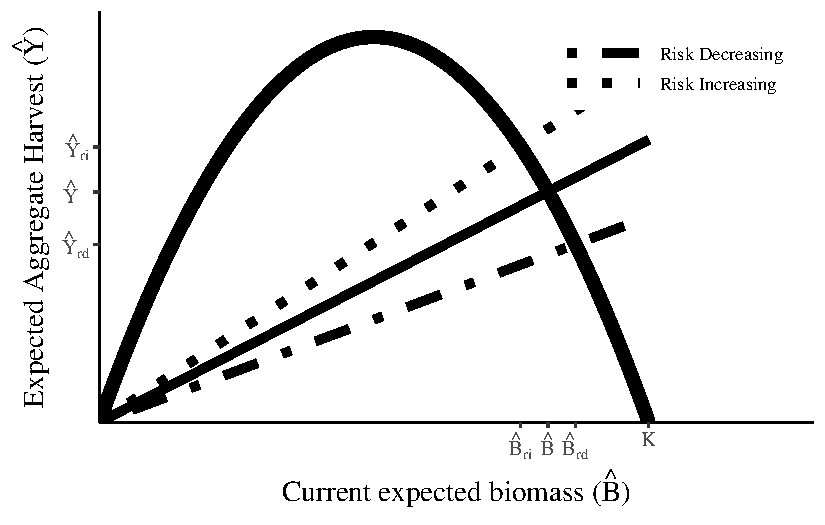
\includegraphics{ibi-behavior_files/figure-pdf/fig-synas-1.pdf}

}

\caption{\label{fig-synas}Equilibrium harvest and biomass levels change
with index insurance depending on the risk effects of inputs. Deviations
from initial harvest allocations (solid line) have different impacts at
levels above and below maximum sustainable yield. Risk decreasing inputs
(long dashes) will always lead to higher equilibrium biomass. Risk
increasing inputs (short dashes) will always lead to lower equilibrium
biomass.}

\end{figure}

Index insurance can lead to conservation benefits in common pool
resources if the production inputs are risk decreasing, but the
implications for harvest depend on the initial bioeconomic equilibrium.
In Figure~\ref{fig-synas}, the first initial bieconomic equilibrium to
the left demonstrates overexploitation with biomass below maximum
sustainable yield. A decrease an effort from index insurance stimulates
faster growth of the stock allowing for more harvest in the future.
Therefore fishers will be more protected from shocks with insurance,
benefit from more current harvest, and there will be a a healthier stock
of fish. Alternatively, if inputs are risk increasing, then index
insurance will shift production to the right lowering harvest and
biomass of the fish pushing the fishery further into overexploitation.

The second initial equilibrium to the right in Figure~\ref{fig-synas} is
underexploited with biomass above maximum sustainable yield. The impact
of index insurance on equilibrium biomass remains the same as when
overexploited by Proposition~\ref{prp-synas}, but the direction of
harvest changes. Now, insurance will lower harvest for risk decreasing
inputs and raise harvest for risk increasing inputs.

Proposition~\ref{prp-synas} offers policymakers a powerful tool to
assess the viability of using index insurance to protect fisheries from
overharvesting and provide conservation benefits. Conservation of common
pool resources through insurance hinges on the risk effects of
production technology. If policymakers are solely interested in
conservation, then only knowing the direction of the fishery risk
effects is necessary. In that case, only fisheries with risk decreasing
inputs should be targeted for index insurance policies. Index insurance
could also be used to incentivize fishing in low capacity communities,
much like how index insurance is used in developing countries to
stimulate agriculture investment. Since most fisheries are overfished,
it is unlikely that a policymaker would target fisheries with risk
increasing inputs with insurance to expand capacity and place more
pressure on the fish stock.

Risk effects remain an elusive concept in fisheries. It is unclear how
to preemptively identify fishery risk effects. Current bioeconomic
models used to study fisheries do not account for risk effects. They are
biased towards risk increasing inputs and therefore will always predict
a lower equilibrium biomass.

Fishery bioeconomic models need to balance complexity in both the
biological and economic systems. More emphasis as been placed on
biological complexity with ecosystem-based management rising in
prevalence. Though some models use Cobb-Douglas and other more flexible
economic production models for harvest, most use a variation of the
Gordon-Schaefer production model. The ability to create a proxy for
stock abundance through catch per unit effort (CPUE), and its simplicity
is why Gordon-Schaefer remains a useful modelling framework for
fisheries. However, Gordon-Schaefer does not allow for flexible risk
effects.

\begin{proposition}[]\protect\hypertarget{prp-gs}{}\label{prp-gs}

Gordon-Schaefer fishery production models with linear harvest and
multiplicative shocks are always risk increasing.

\end{proposition}

\begin{proof}

Risk effects can also be defined as the cross partial of the production
function with respect to input and shock. If positive then an input is
risk increasing, and if negative an input is risk decreasing.

\[
\begin{aligned}
y&=qeB\omega \\
\frac{\partial y}{\partial e \partial \omega} &=qB \\
&>0
\end{aligned}
\]

\end{proof}

Fishery harvest (\(y\)) is a linear function of effort (\(e\)), stock
abundance (\(B\)), and a catchability coefficient (\(q\)) acting as a
measure of technological efficiency. Stock abundance and technological
efficiency are always greater than zero. Without loss of generality,
more sophisticated models will find similar limitations as they are
extensions of the presented simple form. Cobb-Douglas are known to
posses bias towards risk increasing inputs (Just and Pope 1979), and
age-structure models typically use the same linear profit as a
Gordon-Schaefer at each age class with multiplicative environmental
shocks (Tahvonen \emph{et al.} 2018). Fox and Pella-Tomlinson models are
more flexible production models, but each can reduce down to a
Gordon-Schaefer through parameter choice.

Adding insurance to standard bioeconomic fishery models always leads to
an increase in input use by Proposition~\ref{prp-cp}, and a decrease in
equilibrium biomass through Proposition~\ref{prp-synas}. However, these
models were often not designed to account for risk and risk preferences.
Fishers are highly responsive to risk. They mitigate risk through a
variety of measures. Fishers will choose consistent, known fishing
grounds over risking exploring unknown spots (Holland 2008). Fishers
choose to fish less after storms and hurricanes when financial risk is
alleviated by transitioning to catch share programs (Pfeiffer 2020;
Pfeiffer \emph{et al.} 2022). In this context, effort can be seen as an
\emph{income} risk reducing input. If the variability of catch is
reduced, then the pressure to fish to ensure consistent catch is also
reduced.

To date, only one study has quantified risk effects in a fishery
setting. Asche \emph{et al.} (2020) used data from four Norwegian
fishing fleets to measure three input responses to risk. Each fishery
possessed unique mixes of both risk increasing and decreasing inputs.
For example, labor was found to be a risk decreasing input across all
four groups, but only statistically significant in both pelagic seiners.
Capital was risk increasing for coastal seiners and trawlers, but
flipped to risk decreasing for purse seiners and trawlers. Fuel had a
lower, but statistically significant positive risk increasing measure
for three of the four groups.

However, total output variance fluctuated in ways where it was not clear
what the total effect would be. Coastal seiners had significant risk
decreasing effects in labor, but also significant risk increasing
effects in fuel. Overall output variance was insignificantly different
than zero. So while individual inputs impacted risk, overall impacts
were unclear. Index insurance may raise or lower individual inputs
depending on their own unique risk effects, but the overall direction of
conservation cannot be determined. In order to apply the insights gained
from index insurance in a common pool setting to the real world effects
of Asche et al., (2020), our model must be expanded to understand how
index insurance interacts with multiple inputs.

\hypertarget{sec-multi}{%
\section{Insurance with multiple inputs}\label{sec-multi}}

We can use the overarching framework from the previous section and
expand it by adding multiple inputs. To simplify matters, we will focus
on only one fisher, their choice of inputs and insurance, and a set
biomass normalized to one.

Some inputs have varying risk effects. Interaction between inputs risk
effects could change overall impacts from insurance to aggregate harvest
and biomass. Fishers can use a vector of inputs \(X\). Expected mean
production (\(f(X)\)) and variance of outputs (\(h(X)\)) remains the
same. We will use only two inputs, capital and labor, in our model.
Total production thus equals:

\[
\begin{aligned}
y(k,l)=f(k,l)+\omega h(k,l)\\
\text{where }\omega \sim N(0,\sigma^2)
\end{aligned}
\]

As before, random shocks that could be weather or biological shocks is
captured by \(\omega\). Mean production possess classic production
concavity so that \(f'(k,l)>0\) and \(f''(k,l)<0\). Flexible risk
effects imply that \(h'(k,l)\lesseqgtr0\) so that risk increasing
\(h'(k,l)>0\), risk decreasing (\(h'(k,l)<0\)), and no risk effects
\(h'(k,l)=0\). The original specification of Just and Pope make no
assumption on the form of the second derivative of the risk effect
function. To assist signing later on further justification is required.
The marginal impact of adding an input to production variance should
have diminishing effects, because it is impossible to completely
eliminate risk or experience infinite risks. Therefore, when
\(h'(k,l)>0 \rightarrow h''(k,l)<0\), and when
\(h'(k,l)<0 \rightarrow h''(k,l)>0\). The cross partial of risk effects
on production \(\frac{\partial h}{\partial k \partial l}\) must also be
flexible and depend on how inputs interact with each other. For example,
if adding an input does not contribute to the marginal variance of
another input then \(\frac{\partial h}{\partial k \partial l}=0\).
Inputs interactions could be complementary in that adding a risk
decreasing input further enhances the risk reducing properties of the
other inputs, e.g.~(\(\frac{\partial h}{\partial k \partial l}>0\)). In
other instances the inputs may interact counter actively in that adding
more of a risk increasing input might reduce the effect of a risk
decreasing input \(\frac{\partial h}{\partial k \partial l}<0\). In
principle, when inputs share direction of risk effects, their cross
partial ought to be complementary, and otherwise they will be counter
productive.

Costs are convex, \(c'(k,l)>0\) and \(c''(k,l)>0\), in each input.
Prices are constant and set at one so that production and costs together
form random profits.

\begin{equation}\protect\hypertarget{eq-pi}{}{
\pi(k,l)=f(k,l)+\omega h(k,l)-c(k,l)
}\label{eq-pi}\end{equation}

We use the same insurance design from the previous section where
payouts, \(\gamma\), are triggered by \(\omega<0\), and we can partition
profit into good states and bad states. Fishers now maximize expected
utility by selecting both inputs, capital and labor.

\[
F\equiv\max_{k,l}\mathbb{E}[u]=pu(\pi_b(k,l)+(1-p)\gamma)+(1-p)u(\pi_g(k,l)-p\gamma)
\]

Taking the first order conditions yields:

\begin{equation}\protect\hypertarget{eq-foc1}{}{
\begin{aligned}
\frac{\partial F}{\partial k}=(1-p)u'(\pi_g-p\gamma)\frac{\partial \pi_g}{\partial k}+pu'(\pi_b+(1-p)\gamma)\frac{\partial \pi_b}{\partial k} =0\\
\frac{\partial F}{\partial l}=(1-p)u'(\pi_g-p\gamma)\frac{\partial \pi_g}{\partial l}+pu'(\pi_b+(1-p)\gamma)\frac{\partial \pi_b}{\partial l} =0
\end{aligned}
}\label{eq-foc1}\end{equation}

Given the existence of the first order condition, we can use the
implicit function theorem (IFT) to look at the impact of an exogenous
variable change locally at the solution. In other words, using IFT will
clarify how a change to the insurance parameter \(\gamma\) will lead to
new allocations of captial and labor. We can differentiate
Equation~\ref{eq-foc1} with respect to \(\gamma\) by the chain rule.
This yields:

\[
\begin{pmatrix}
\frac{\partial F}{\partial k \partial k} & \frac{\partial F}{\partial k \partial l} \\
\frac{\partial F}{\partial l \partial k} & \frac{\partial F}{\partial l \partial l}
\end{pmatrix}
\begin{pmatrix}
\frac{\partial k^*}{\partial \gamma} \\
\frac{\partial l^*}{\partial \gamma}
\end{pmatrix}
=-\begin{pmatrix}
\frac{\partial F}{\partial k \partial \gamma} \\
\frac{\partial F}{\partial l \partial \gamma}
\end{pmatrix}
\]

Inverting the Hessian matrix to the other side allows us to isolate the
effects on the optimal allocations.

\begin{equation}\protect\hypertarget{eq-opt2}{}{
\begin{pmatrix}
\frac{\partial k^*}{\partial \gamma} \\
\frac{\partial l^*}{\partial \gamma}
\end{pmatrix}
=-
\begin{pmatrix}\frac{\partial F}{\partial k \partial k} & \frac{\partial F}{\partial k \partial l} \\
\frac{\partial F}{\partial l \partial k} & \frac{\partial F}{\partial l \partial l}
\end{pmatrix}^{-1}
\begin{pmatrix}
\frac{\partial F}{\partial k \partial \gamma} \\
\frac{\partial F}{\partial l \partial \gamma}
\end{pmatrix}
}\label{eq-opt2}\end{equation}

Crammer's rule allows us to solve this system of equations so long as
the determinant of the system is not equal to 0. Luckily, the
determinant is a 2x2 hessian of a concave maximization problem. By
definition it is strictly positive. Applying Crammer's rule to
Equation~\ref{eq-opt2} gives us:

\[
\begin{pmatrix}
\frac{\partial k^*}{\partial \gamma} \\
\frac{\partial l^*}{\partial \gamma}
\end{pmatrix}
=\frac{-1}{Det}
\begin{pmatrix}\frac{\partial F}{\partial l \partial l} & \frac{-\partial F}{\partial k \partial l} \\
\frac{-\partial F}{\partial l \partial k} & \frac{\partial F}{\partial k \partial k}
\end{pmatrix}
\begin{pmatrix}
\frac{\partial F}{\partial k \partial \gamma} \\
\frac{\partial F}{\partial l \partial \gamma}
\end{pmatrix}
\]

Solving the systems yields:

\begin{equation}\protect\hypertarget{eq-ivtsol}{}{
\begin{aligned}
&\frac{\partial k}{\partial \gamma}=\frac{-1}{Det}\left[\frac{\partial F}{\partial l \partial l}\frac{\partial F}{\partial k \partial \gamma}-\frac{\partial F}{\partial k \partial l}\frac{\partial F}{\partial l \partial \gamma}\right] \\
&\frac{\partial l}{\partial \gamma}=\frac{-1}{Det}\left[\frac{-\partial F}{\partial l \partial k}\frac{\partial F}{\partial k \partial \gamma}+\frac{\partial F}{\partial k \partial k}\frac{\partial F}{\partial l \partial \gamma}\right]
\end{aligned}
}\label{eq-ivtsol}\end{equation}

Because the determinate will always be positive by the definition of the
second order condition, we can focus on the interior of the brackets. If
positive (negative), then insurance will lower (raise) use of that
input. To sign Equation~\ref{eq-ivtsol}, we need to determine the
partial derivatives. All six partials are included in the appendix. All
the partials help define the impact of insurance on multiple input use.

Fishers must be risk averse, and inputs must contribute to risk
management in some way. Otherwise, there will be no impact on insurance.

\begin{proposition}[]\protect\hypertarget{prp-rn}{}\label{prp-rn}

Risk neutral fishers will not change their input use with index
insurance

\end{proposition}

\begin{proof}

Risk neutrality implies that \(u'(k,l)=0\) and \(u''(k,l)=0\). Subbing
\(u''(k,l)=0\) into both Equation~\ref{eq-kgam} and
Equation~\ref{eq-lgam} forces them to both equal zero. Plugging zero for
\(\frac{\partial F}{\partial l \partial \gamma}\) and
\(\frac{\partial F}{\partial k \partial \gamma}\) into
Equation~\ref{eq-ivtsol} makes both elements also zero in the interior.
Thus risk neutral fishers would not change input allocation with the
addition of index insurance.

\end{proof}

To help prove the remaining propositions, the following corollary will
be valuable.

\begin{corollary}[]\protect\hypertarget{cor-mp}{}\label{cor-mp}

Marginal profit in the bad state of the world is greater (less) than
marginal profit in the good state for risk decreasing (increasing)
inputs. If inputs have zero risk effects, the marginal profits are
equivalent in both states.

\end{corollary}

The proof is included in the appendix.

\begin{proposition}[]\protect\hypertarget{prp-rezero}{}\label{prp-rezero}

Index insurance will not change the input allocations when all inputs
possess no risk effects.

\end{proposition}

\begin{proof}

The second part of Corollary~\ref{cor-mp} states that the marginal
profits across states are equal. If the marginal profits across states
are equal, then in Equation~\ref{eq-kgam} and Equation~\ref{eq-lgam} the
weight between positive and negative utilities is also equal and cancel
out leading to Equation~\ref{eq-kgam} and Equation~\ref{eq-lgam} both
equaling zero. Plugging zeros into Equation~\ref{eq-ivtsol} for the
insurance partials leads to an interior zero and no change in input use.

\end{proof}

Risk averse fishers will buy actuarially fair insurance. If the inputs
possess risk effects then they will lead to changes in the input.
Proposition~\ref{prp-samre} defines the change in multiple inputs
simultaneously with insurance.

\begin{proposition}[]\protect\hypertarget{prp-samre}{}\label{prp-samre}

With multiple inputs, index insurance will raise (lower) use of risk
increasing (decreasing) inputs in accordance to an inputs individual
risk effects when the following sufficient condition is true:

\(\frac{\partial F}{\partial k\partial l}>0\) when both inputs share the
same risk effects, and \(\frac{\partial F}{\partial k\partial l}<0\)
when inputs have opposite risk effects.

Otherwise, Index Insurance will have ambiguous effects on each input
allocation.

\end{proposition}

\begin{proof}

Corollary~\ref{cor-mp} allows us to sign Equation~\ref{eq-kgam} and
Equation~\ref{eq-lgam} for any risk effect on either input. Concave
utility by definition leads to \(u''<0\). For simplicity, we'll only
focus on Equation~\ref{eq-kgam}, but all applies equally to
Equation~\ref{eq-lgam}. Insurance payouts equalize profits between
different states. If insurance completely covers all loss, then we can
rewrite equation Equation~\ref{eq-kgam} as

\begin{equation}\protect\hypertarget{eq-kgamsol}{}{
\frac{\partial F}{\partial k \partial \gamma}=\overbrace{\overbrace{(1-p)pu''(\cdot)}^{-}\overbrace{[\frac{\partial \pi_b}{\partial k}-\frac{\partial \pi_g}{\partial k}]}^{-}}^{+}
}\label{eq-kgamsol}\end{equation}

Corollary~\ref{cor-mp} allows us to sign the interior brackets of
Equation~\ref{eq-kgamsol}. Risk increasing (decreasing) inputs make the
interior negative (positive). Thus, when an input is risk increasing
(decreasing), we can sign Equation~\ref{eq-kgam} and
Equation~\ref{eq-lgam} as positive (negative). Equation~\ref{eq-kk} and
Equation~\ref{eq-ll} will always be negative due to concave utility.

Suppose both inputs are risk increasing so Equation~\ref{eq-kgam} and
Equation~\ref{eq-lgam} are positive. The only way for
Equation~\ref{eq-ivtsol} to be unambiguously positive is for
Equation~\ref{eq-crossl} and Equation~\ref{eq-crossk} to be positive.

\[
\begin{aligned}
&\frac{\partial k}{\partial \gamma}=\overbrace{\frac{-1}{Det}}^{-}\left[\overbrace{\overbrace{\frac{\partial F}{\partial l \partial l}}^{-}\overbrace{\frac{\partial F}{\partial k \partial \gamma}}^{+}\overbrace{-\frac{\partial F}{\partial k \partial l}}^{-}\overbrace{\frac{\partial F}{\partial l \partial \gamma}}^{+}}^{-}\right] >0\\
&\frac{\partial l}{\partial \gamma}=\overbrace{\frac{-1}{Det}}^{-}\left[\overbrace{\overbrace{\frac{-\partial F}{\partial l \partial k}}^{-}\overbrace{\frac{\partial F}{\partial k \partial \gamma}}^{+}+\overbrace{\frac{\partial F}{\partial k \partial k}}^{-}\overbrace{\frac{\partial F}{\partial l \partial \gamma}}^{+}}^{-}\right]>0
\end{aligned}
\]

Both risk increasing inputs will be raised with index insurance. The
results hold for risk decreasing inputs as the overall signs flip. Risk
decreasing inputs will be lowered with index insurance.

Now suppose inputs have mixed risk effects. For simplicity, capital will
be risk increasing and labor will be risk decreasing. The results will
hold for the opposite case. By Corollary~\ref{cor-mp},
Equation~\ref{eq-kgam} is positive, while Equation~\ref{eq-lgam} is
negative. Equation~\ref{eq-ivtsol} will be unambiguously positive if
Equation~\ref{eq-crossl} and Equation~\ref{eq-crossk} are negative.

\[
\begin{aligned}
&\frac{\partial k}{\partial \gamma}=\overbrace{\frac{-1}{Det}}^{-}\left[\overbrace{\overbrace{\frac{\partial F}{\partial l \partial l}}^{-}\overbrace{\frac{\partial F}{\partial k \partial \gamma}}^{+}\overbrace{-\frac{\partial F}{\partial k \partial l}}^{+}\overbrace{\frac{\partial F}{\partial l \partial \gamma}}^{-}}^{-}\right] >0\\
&\frac{\partial l}{\partial \gamma}=\overbrace{\frac{-1}{Det}}^{-}\left[\overbrace{\overbrace{\frac{-\partial F}{\partial l \partial k}}^{+}\overbrace{\frac{\partial F}{\partial k \partial \gamma}}^{+}+\overbrace{\frac{\partial F}{\partial k \partial k}}^{-}\overbrace{\frac{\partial F}{\partial l \partial \gamma}}^{-}}^{+}\right]<0
\end{aligned}
\]

The risk increasing input will be raised with index insurance, while the
risk decreasing input will be lowered.

\end{proof}

Proposition~\ref{prp-samre} shows that index insurance can have clear
impacts even in complex settings with multiple inputs provided the
sufficient condition holds. However, it is not clear ex-ante what the
sign of the cross partial inputs of the first order condition should be.
Equation~\ref{eq-crossl} and Equation~\ref{eq-crossk} themselves could
be ambiguous. Rearranging Equation~\ref{eq-crossl} and
Equation~\ref{eq-crossk} shows that the relative weight between the
marginal profits of each input \(\frac{\partial f}{\partial k}\) and the
risk effects cross partial \(\frac{\partial h}{\partial k \partial l}\)
will determine the overall sign of the first order cross partials.
Essentially, fishers change their inputs depending on whether a given
input makes the other input more productive than the risk it adds.
Dividing Equation~\ref{eq-crossk} by \(-\frac{u'}{u'}\) allows us to
rearrange terms to show the tension between mean production and risk
effects.

\begin{equation}\protect\hypertarget{eq-crosssolve}{}{
\begin{aligned}
-\frac{\partial F}{\partial k \partial l}&=(1-p)u'\frac{-u''}{u'}\frac{\partial \pi_g}{\partial k}\frac{\partial \pi_g}{\partial l}-(1-p)u'\frac{\partial \pi_g}{\partial k\partial l}\frac{u'}{u'}\\
&+ pu'\frac{\partial \pi_b}{\partial k}\frac{\partial \pi_b}{\partial l}\frac{-u''}{u'}-pu'\frac{\partial \pi_b}{\partial k \partial l}\frac{u'}{u'}\\
&=(1-p)u'[\frac{-u''}{u'}]\frac{\partial \pi_g}{\partial k}\frac{\partial \pi_g}{\partial l}+pu'[\frac{-u''}{u'}]\frac{\partial \pi_b}{\partial k}\frac{\partial \pi_b}{\partial l}\\
&-(1-p)u'\frac{\partial \pi_g}{\partial k\partial l}-pu'\frac{\partial \pi_b}{\partial k \partial l}
\end{aligned}
}\label{eq-crosssolve}\end{equation}

The concavity of profit with positive risk aversion \(\frac{-u''}{u'}\)
lead line 3 in Equation~\ref{eq-crosssolve} to be positive. The cross
partials in line 4 paint a more complicated picture. Whether inputs
enhance or reduce the risk effect qualities of each other influences the
weight of line 4. When inputs share risk effects, they ought to increase
the risk effects of each other so that
\(\frac{\partial h}{\partial k \partial l}>0\). Therefore line 4 in
Equation~\ref{eq-crosssolve} becomes more negative as all terms are
positive. It is relatively more likely that Equation~\ref{eq-crosssolve}
is negative when risk effects are shared.

When risk effects are mixed, with one input increasing and one input
decreasing, the risk effects counteract each other
\(\frac{\partial h}{\partial k \partial l}<0\). Line 4 in
Equation~\ref{eq-crosssolve} becomes relatively less negative. If the
difference between the risk effects cross partial
\(\frac{\partial h}{\partial k \partial l}\) outweigh the mean
production cross partial \(\frac{\partial f}{\partial k \partial l}\)
then line 4 becomes unambiguously becomes positive. Then
\(-\frac{\partial F}{\partial k \partial l}>0\) and
\(-\frac{\partial F}{\partial l \partial k}>0\). The relative changes
with complimentary or counteractive risk effects matches the signs
needed for the condition in Proposition~\ref{prp-samre} to hold.

Despite the seemingly rigid conditions, Proposition~\ref{prp-samre} is
quite powerful. It states that the direction all inputs should change is
based solely on the characteristics of their own risk effects. Other
inputs may influence the magnitude of change, but the direction is
unequivocal. It remains unclear how much overall harvest will change.
Simulations show the total impact on harvest can vary substantially, and
that the conditions to ensure unambiguous change can be met. Though when
applied with real world estimates of risk effects, the conditions may
not hold and the effects of index insurance may not follow simple rules.

\hypertarget{sec-sim}{%
\section{Numerical Simulations}\label{sec-sim}}

We use a simple numerical simulation to test the necessary conditions in
Proposition~\ref{prp-samre} and to determine the magnitude of change in
input use for Norwegian fisheries using the parameters found in Asche
\emph{et al.} (2020). First, we present the simulations from the two
input case to gain additional insight into how index insurance changes
multiple inputs. Fisher earn profit through harvest with a Just and Pope
production function with mean biomass normalized to one, and convex cost
function.

\begin{equation}\protect\hypertarget{eq-sim}{}{
\pi(k,l)=\hat{B}k^{\alpha_k}l^{\alpha_l}+\omega k^{\beta_k}l^{\beta_l}-c_kk^2-c_ll^2
}\label{eq-sim}\end{equation}

Random shocks (\(\omega\)) are distributed normally with a mean of zero
and a standard deviation of \(\sigma_w\). Capital (\(k\)) and labor
(\(l\)) have both mean production elasticities (\(\alpha_k\) and
\(\alpha_l\)) and flexible risk elasticities (\(\beta_k\) and
\(\beta_l\)). Fishers choose both capital and labor to maximize expected
utility. We use a constant absolute risk aversion utility function.

Multiple index insurance policies are tested through changes in coverage
and trigger levels. One scenario set constant payout amounts at 50\% of
pre-insurance profit and the other allows fishers to choose payouts.
Trigger levels are set to engage at any below average weather, shocks of
more than 75\% loss, and catastrophic shocks that reduce biomass below
90\%. All premiums are actuarilly fair. We vary fisher production
parameters and risk aversion to create a comprehensive dataset of
possible combinations. Risk effects vary between -0.7 and 0.7 with
iterative increases of 0.1 ignoring situations of 0 risk effects.
Fishers can posses low, medium, and high mean elasticity values
\(\alpha\in\{0.25,0.5,0.75\}\). Coefficient of constant absolute risk
aversion ranges from 1 to 3. Within each scenario, a Monte Carlo
simulation creates 1000 weather random weather shocks with three
variants of standard deviation \(\sigma_w\in\{0.33,0.66,1\}\).

\hypertarget{numerical-simulation-results}{%
\subsection{Numerical simulation
results}\label{numerical-simulation-results}}

Increasing insurance incentivizes fishers to use more risk decreasing
inputs and less risk increasing inputs (Figure~\ref{fig-ins}). The
conditions of Proposition~\ref{prp-samre} can be satisfied with CARA
utility, a Just-Pope Production function, and normal values of mean and
risk elasticities. Index insurance also increases utility shown by the
green lines in Figure~\ref{fig-ins}, but there exists an optimal amount
of insurance coverage for fishers. The optimal values of insurance are
generally lower when fishers use risk decreasing inputs. The inputs and
insurance act as substitutes for each other both lowering the variance
of income fishers experience.

\begin{figure}

{\centering 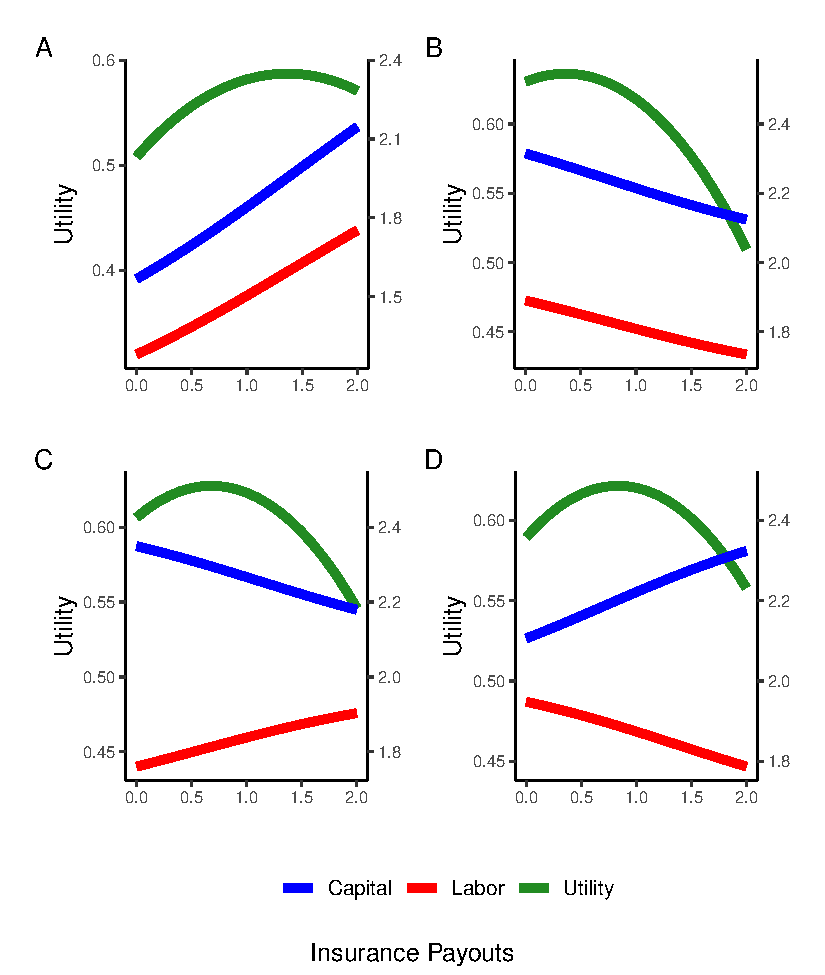
\includegraphics{ibi-behavior_files/figure-pdf/fig-ins-1.pdf}

}

\caption{\label{fig-ins}Fisher utility (green line) is concave in
insurance payouts. Inputs change in accordance to their individual risk
effects. The secondary y-axis shows input allocations for capital (blue
line) and labor (red line). Panel A has both inputs with positive risk
effects (\(\beta=0.5\)). Panel B has both inputs with negative risk
effects (\(\beta=-0.5\)). Panel C shows the effects when capital is a
risk decreasing input (\(\beta=- 0.5\)) while labor is risk increasing
(\(\beta=0.5\)). Panel D flips the risk effects of capital and labor.}

\end{figure}

Figure~\ref{fig-ins} shows that conditions of
Proposition~\ref{prp-samre} can be satisfied, but it does not show the
conservation outcomes of index insurance. Fishers use the new allocation
of inputs to change their overall harvest and thus impact on the biomass
of fish stocks. Harvest changes are influenced by the relative
combination of risk effects, mean production elastiticies, and the
amount of insurance. Fishers reduce harvest more aggressively with risk
decreasing inputs when offered a set contract of 50\% coverage of
pre-insurance profits (Panel A) relative to their optimal choice (Panel
B) (Figure~\ref{fig-multi-h-even}). Allowing fishers to choose their
insurance coverage leads them to increase harvest more with risk
increasing inputs. This phenomenon relates back to Figure~\ref{fig-ins}.
A 50\% coverage is an overinvestment in insurance for risk decreasing
inputs and an underinvestment for risk increasing inputs.

Mixed risk effects reduce the overall impact on harvest. The more
flexible risk parameter dominates the less flexible one in terms of
which input reduces overall harvest shown in the top left and bottom
right quadrants of both panels in Figure~\ref{fig-multi-h-even}.

\begin{figure}

{\centering 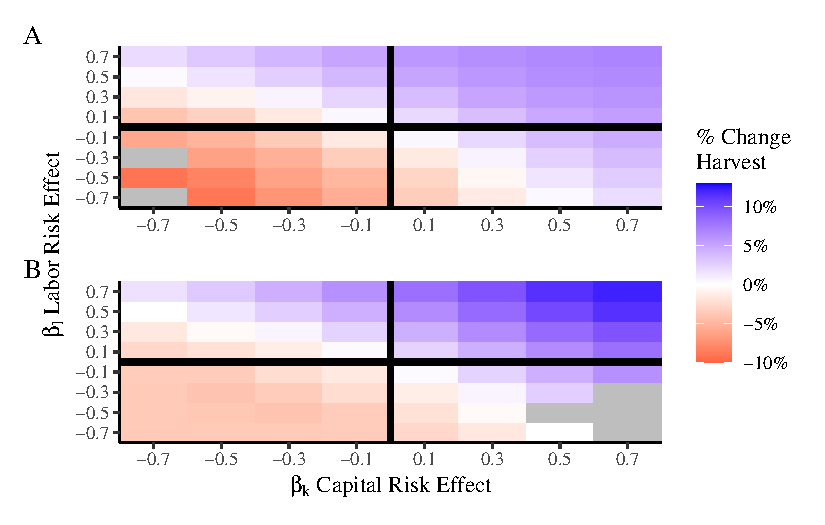
\includegraphics{ibi-behavior_files/figure-pdf/fig-multi-h-even-1.pdf}

}

\caption{\label{fig-multi-h-even}Percent Change in fishing harvest when
fishers use index insurance with low mean elasticity values
(\(\alpha_{k,l}=0.25\)). In Panel A, Insurance payouts are a set
variable. In Panel B, fishers choose insurance payouts. Red colors show
overall decreases in harvest while blue colors show overall increases in
harvest.}

\end{figure}

Increasing the mean elasticities exacerbates the discrepancies between
allowing fishers to choose insurance payouts versus receiving a set
amount. When the productivity of harvest (\(\alpha\)) is higher, the
tradeoff between reducing variance and catch changes. Though insurance
protects against risk, lowering the use of risk reducing inputs looses
more mean catch with higher production elasticities. Fishers reduce
aggregate harvest less with risk reducing inputs when mean elasticities
are high. The opposite is true for risk increasing inputs. Insurance
protects against the variance of adding more inputs and fishers receive
a greater mean catch.

\begin{figure}

{\centering 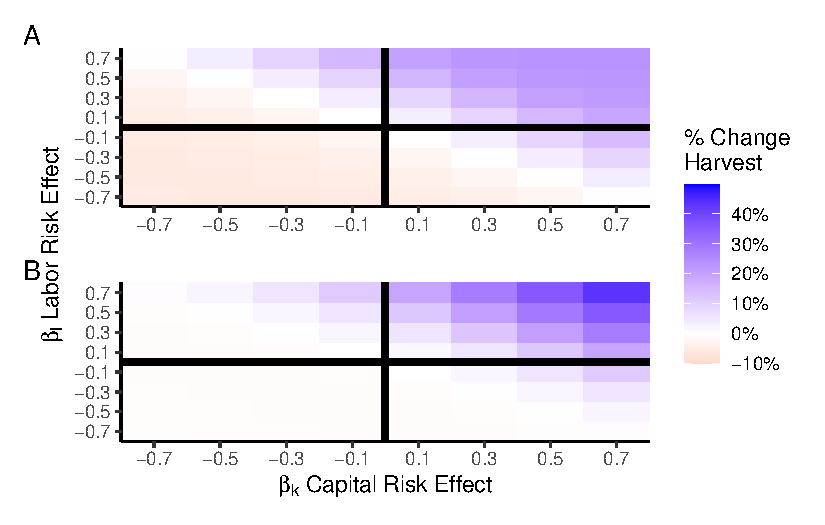
\includegraphics{ibi-behavior_files/figure-pdf/fig-multi-h-even-hi-1.pdf}

}

\caption{\label{fig-multi-h-even-hi}When fishers choose insurnace, they
drastically increase (blue) harvest with risk increasing relative to no
insurance harvest. Inputs share the same mean elasticity
(\(\alpha_{k,l}=0.5\)). Insurance payouts are a choice variable. Risk
aversion is set to 1. Weather variance is 0.5}

\end{figure}

\hypertarget{application-to-real-world-fisheries}{%
\subsection{Application to Real World
Fisheries}\label{application-to-real-world-fisheries}}

Asche et al., (2020) aggregated by vessel type and not species, so there
is no reasonable estimate for biomass. They accounted for biomass using
fixed effects in their regression, but without additional information,
our simulations normalize biomass to 1 and only focus on the relative
change in inputs and aggregate harvest. The simulation model extends the
two input case to include fuel (\(f\)).

\begin{equation}\protect\hypertarget{eq-sim3}{}{
\pi(k,l)=k^{\alpha_k}l^{\alpha_l}f^{\alpha_f}+\omega k^{\beta_k}l^{\beta_l}-c_kk^2-c_ll^2-c_ff^2
}\label{eq-sim3}\end{equation}

Table~\ref{tbl-asche} shows the production and risk elasticities of the
four vessel types used in the simulation. While not all elasticities
were found to be statistically different from zero, we used their raw
values because dropping only those variables that are significant in
both matching parameters would have kept only a few valid combinations.
All non-significant elasticities led to small changes as expected, but
their interactions with other inputs could partially drive some of the
observed outcomes.

\hypertarget{tbl-asche}{}
\begin{longtable}[]{@{}
  >{\raggedright\arraybackslash}p{(\columnwidth - 12\tabcolsep) * \real{0.2410}}
  >{\raggedleft\arraybackslash}p{(\columnwidth - 12\tabcolsep) * \real{0.1325}}
  >{\raggedleft\arraybackslash}p{(\columnwidth - 12\tabcolsep) * \real{0.1325}}
  >{\raggedleft\arraybackslash}p{(\columnwidth - 12\tabcolsep) * \real{0.1325}}
  >{\raggedleft\arraybackslash}p{(\columnwidth - 12\tabcolsep) * \real{0.1205}}
  >{\raggedleft\arraybackslash}p{(\columnwidth - 12\tabcolsep) * \real{0.1205}}
  >{\raggedleft\arraybackslash}p{(\columnwidth - 12\tabcolsep) * \real{0.1205}}@{}}
\caption{\label{tbl-asche}Production and Risk elasticities of Norwegian
Fisheries}\tabularnewline
\toprule\noalign{}
\begin{minipage}[b]{\linewidth}\raggedright
\end{minipage} & \begin{minipage}[b]{\linewidth}\raggedleft
\(\alpha_k\)
\end{minipage} & \begin{minipage}[b]{\linewidth}\raggedleft
\(\alpha_l\)
\end{minipage} & \begin{minipage}[b]{\linewidth}\raggedleft
\(\alpha_f\)
\end{minipage} & \begin{minipage}[b]{\linewidth}\raggedleft
\(\beta_k\)
\end{minipage} & \begin{minipage}[b]{\linewidth}\raggedleft
\(\beta_l\)
\end{minipage} & \begin{minipage}[b]{\linewidth}\raggedleft
\(\beta_f\)
\end{minipage} \\
\midrule\noalign{}
\endfirsthead
\toprule\noalign{}
\begin{minipage}[b]{\linewidth}\raggedright
\end{minipage} & \begin{minipage}[b]{\linewidth}\raggedleft
\(\alpha_k\)
\end{minipage} & \begin{minipage}[b]{\linewidth}\raggedleft
\(\alpha_l\)
\end{minipage} & \begin{minipage}[b]{\linewidth}\raggedleft
\(\alpha_f\)
\end{minipage} & \begin{minipage}[b]{\linewidth}\raggedleft
\(\beta_k\)
\end{minipage} & \begin{minipage}[b]{\linewidth}\raggedleft
\(\beta_l\)
\end{minipage} & \begin{minipage}[b]{\linewidth}\raggedleft
\(\beta_f\)
\end{minipage} \\
\midrule\noalign{}
\endhead
\bottomrule\noalign{}
\endlastfoot
Coastal Seiners & 0.294 & 0.421 & 0.457 & 0.184 & -0.432 & 0.119 \\
Coastal Groundfish & 0.463 & 0.421 & 0.355 & 0.965 & -0.080 & 0.113 \\
Purse Seiners & 0.941 & -0.108 & 0.605 & -0.454 & -0.231 & 0.160 \\
Groundfish Trawlers & 0.210 & 0.106 & 0.531 & -2.788 & -0.110 &
-0.024 \\
\end{longtable}

Index insurance in Norwegian fisheries would have lead to changes in
input use and overall harvest. Table~\ref{tbl-nor} shows that index
insurance would have lead to a maximum change of 15\% in total harvest
for the coastal groundfish fishery. This was primarily driven by large
increases in capital (20.36\%) and fuel (8.89\%). All inputs had
relatively similar mean production elasticities, but capital was
strongly risk increasing with the highest positive risk elasticity.
Labor was a risk decreasing input, but also rose with insurance. This is
an example where the conditions of Proposition~\ref{prp-samre} do not
hold. The large discrepancy in production risk elastiticites is probably
a reason for this in addition to the interactions terms at play by
adding a third input. The chosen insurance payout was also much higher
than the other vessel types. This reflects the observation from
Figure~\ref{fig-ins} that that fishers choose higher levels of insurance
coverage as a means to substitute the additional risk they are taking
with expanded production.

Purse seiners saw the largest reduction in overall harvest. Capital for
purse seiners is the most productive input out of all fisheries and
inputs. Because it is risk reducing, it dominates the slightly risk
increasing fuel input to lead the entire fishery to reduce harvest by
6.3\%. this shows another violation of Proposition~\ref{prp-samre}. In
the opposite direction this time. Labor allocations did not change. No
labor was allocated in either optimal choice, because the production
elasticity was negative. Insurance payouts were also higher than the
other fisheries that saw reductions. The high productivity of capital
and fuel were most likely driving this result because small reductions
in these productive inputs needed larger compensations.

Coastal seiners are perhaps the most intriguing outcome, because all
parameters were significant and shows the conditions for
Proposition~\ref{prp-samre} can hold in the real world with multiple
inputs. All input use changes followed their respective risk effects.
Capital (0.44\%) and fuel (0.11\%) both increased, while labor (-1.01\%)
decreased. In aggregate, there was a small reduction in harvest (0.3\%).
While insurance lead to a change, it was rather small and would not have
a large impact on the fishery. The counteractive effects of the risk
effects may negate some of the desire to change production as insurance
incentivizes both increases and decreases in harvest.

Inputs in the groundfish trawler industry were all risk reducing.
Unsurprsingly, each input saw a reduction in use when index insurance
was offered. Capital was exremely risk reducing and saw a 4.14\%
reduction in use, but was a relatively less productive input so overall
harvest changed by only 1.4\%. Inusrance payouts were selected to be low
as seen in the two input simulations with risk decreasing inputs.

\hypertarget{tbl-nor}{}
\begin{longtable}[]{@{}
  >{\raggedright\arraybackslash}p{(\columnwidth - 10\tabcolsep) * \real{0.2597}}
  >{\raggedright\arraybackslash}p{(\columnwidth - 10\tabcolsep) * \real{0.1039}}
  >{\raggedright\arraybackslash}p{(\columnwidth - 10\tabcolsep) * \real{0.1039}}
  >{\raggedright\arraybackslash}p{(\columnwidth - 10\tabcolsep) * \real{0.0909}}
  >{\raggedright\arraybackslash}p{(\columnwidth - 10\tabcolsep) * \real{0.1039}}
  >{\raggedleft\arraybackslash}p{(\columnwidth - 10\tabcolsep) * \real{0.3377}}@{}}
\caption{\label{tbl-nor}Application of Index Insurance to risk effect
parameters of Norwegian Fisheries}\tabularnewline
\toprule\noalign{}
\begin{minipage}[b]{\linewidth}\raggedright
\end{minipage} & \begin{minipage}[b]{\linewidth}\raggedright
Capital
\end{minipage} & \begin{minipage}[b]{\linewidth}\raggedright
Labor
\end{minipage} & \begin{minipage}[b]{\linewidth}\raggedright
Fuel
\end{minipage} & \begin{minipage}[b]{\linewidth}\raggedright
Harvest
\end{minipage} & \begin{minipage}[b]{\linewidth}\raggedleft
Insurance Payout \(\gamma\)
\end{minipage} \\
\midrule\noalign{}
\endfirsthead
\toprule\noalign{}
\begin{minipage}[b]{\linewidth}\raggedright
\end{minipage} & \begin{minipage}[b]{\linewidth}\raggedright
Capital
\end{minipage} & \begin{minipage}[b]{\linewidth}\raggedright
Labor
\end{minipage} & \begin{minipage}[b]{\linewidth}\raggedright
Fuel
\end{minipage} & \begin{minipage}[b]{\linewidth}\raggedright
Harvest
\end{minipage} & \begin{minipage}[b]{\linewidth}\raggedleft
Insurance Payout \(\gamma\)
\end{minipage} \\
\midrule\noalign{}
\endhead
\bottomrule\noalign{}
\endlastfoot
Coastal Seiners & 0.44\% & -1.011\% & 0.11\% & -0.3\% & 0.43 \\
Coastal Groundfish & 20.36\% & 6.578\% & 8.89\% & 15.4\% & 1.24 \\
Purse Seiners & -4.39\% & 0.000\% & -3.77\% & -6.3\% & 0.81 \\
Groundfish Trawlers & -4.14\% & -0.979\% & -0.69\% & -1.4\% & 0.23 \\
\end{longtable}

\hypertarget{sec-disc}{%
\section{Discussion}\label{sec-disc}}

Our paper is the first to investigate the interaction of risk effects
and index insurance in a common pool resource. We emphasize a fishery
setting due to burgeoning policy considerations and unique
characteristics of fisheries that merit deeper elucidation. Index
insurance has the potential to alleviate overfishing pressures in common
pool fisheries, but it depends on the inputs risk effects. Risk effects
control the direction and impact of index insurance on input use and
harvest. Standard fishery models implicitly assume all inputs are risk
increasing. Thus, applying index insurance in standard models will
always lead to increases in fishing effort and reductions in stock
biomass.

Risk effects need to be reconciled in a fisheries setting, particularly
risk decreasing inputs. Crop covers and pesticide provide clear examples
in agriculture, but what do risk decreasing inputs look like in
fisheries? Asche \emph{et al.} (2020) provide empirical evidence of the
existence of risk decreasing inputs, but do not elaborate on why or how
labor and capital directly decrease risk. Labor is perhaps the more
intuitive risk decreasing input. Technical expertise of crew and
captains can hedge against luck when fishing (Alvarez \emph{et al.}
2006). Better trained crew can deploy gear in a safe and timely manner,
increasing the likelihood of effective sets.

Capital is a more complex input, because it can be both risk increasing
and decreasing. Capital investments in fisheries typically refer to
vessel tonnage, engine power, and gear technology The spatiotemporal
dimension of fishing decisions may explain how capital can potentially
possess both risk effects. Fishers have to make decisions on where,
when, and how long to fish that differ from the set grids of agriculture
(Reimer \emph{et al.} 2017). Capital offers protection from risk by
allowing fishers to explore more fishing grounds, use more secure gear,
and fish in more adverse weather conditions. When common pool resources
incentivize the race to fish, having larger vessels may be a risk
reducing input as the sooner a fisher can catch they assure their income
at the expense of other fishers. Adding risk aversion to standard models
of common pool fisheries suggests fishers should lower their capital use
compared to risk neutral allocations (Mesterton-Gibbons 1993; Tilman
\emph{et al.} 2018). Yet, overcapitalization and overfishing are more
often observed in the real world. Either fishers are never risk averse
or the risk effects of capital are not as simple as the standard model
suggests. When capital is allowed to be a risk decreasing, optimal
allocations are much higher than risk neutral equilibrium suggesting
fishers are making rational, risk averse decisions.

The transfer between inputs and insurance reflects the substitution
between self-insurance and formal insurance (Quaas and Baumgärtner
2008). If index insurance is designed to reduce fishing capacity,
efforts must be made to ensure that it does not take away from the self
resiliency of fishers. Labor appears to be consistently risk reducing
and acts as a form of self insurance. If index insurance incentivizes
captains to hire less crew, the stock of fish may be preserved, but less
employment may reverberate throughout the community. Fishing is often a
primary employment opportunity in coastal communities. Lowering
employment options may lead to increased poverty or concentrated wealth.
The resiliency of the community would be compromised rather than
enhanced. The same idea applies to capital. If fishers are overinvesting
in capital to hedge against some form of risk, policymakers need to be
sure the insurance is replacing maladaptive self insurance behavior.

The primary form of self insurance in fisheries is management. To this
point our analysis explicitly modeled scenarios without the existence of
management. Most fisheries are managed in some form. The interaction
between management and insurance may be complementary or substitutes.
For example, well managed fisheries that have responsive harvest control
rules may not need insurance. The management system is already providing
the necessary risk protection. Insurance demand and uptake may be low in
these fisheries. Insurance may also complement management to provide the
financial relief that management cannot offer. Managers often focus on
the biological health of the fishery that can run at odds with fishers
desire to enhance their income. Insurance can act as the financial
relief and allow managers to pursue more active strategies to protect
fish stocks without political resistance from lowered quotas. The
interaction between insurance and management requires further
investigation especially with the the numerous management strategies
that exist in fisheries.

Design and access of insurance must also consider equity. The current
federal disaster relief program is inequitable with bias towards large
industrial vessels (Jardine \emph{et al.} 2020). Replacing the program
with an equally inequitable program would be foolhardy. Current US farm
subsidies, including insurance premiums, are heavily skewed towards
large agribusinesses (White and Hoppe 2012). Dimensions of access,
procedural, representation, and distribution must all be built into the
design of new fishery index insurance programs (Fisher \emph{et al.}
2019). For example, small scale fishers may have income constraints that
prevent them from buying the initial contract. Microfinance options
connected to insurance have been used in agriculture to alleviate this
burden to some success (Dougherty \emph{et al.} 2021). Additionally, we
must ensure that is not only the vessel owners who reap the benefits of
insurance. Deckhands and crew are laid off during closures. If index
insurance payouts are going through the entire fishery, the most
vulnerable to closures must be protected as well. Contract stipulations
could mandate that only cost expenses are covered by payouts thereby
including lost wages to the crew. Agriculture contracts often are
designed to directly cover expenses.

Our model only directly models behavior change through moral hazards.
Index insurance could be designed to incentivize other forms of
sustainable behavior change. We define three pathways insurance can
change behavior: Moral hazards, Quid Pro Quo, and Collective Action.
Moral hazards were proven in this paper to have ambiguous impacts
controlled by the risk characteristics of fisher inputs.

Quid Pro Quo is the idea that insurance contracts could be designed with
conservation measures built in. Fishers would be required to adopt
sustainable practices in order to qualify for insurance. Quid Pro Quo is
already used in agricultural insurance in the form of Good Farm
Practices. Farmers must submit management plans to US Risk Management
Agency that clearly outline their conservation practices in order to
qualify for insurance. Working closely with management agencies,
insurance companies could design contracts that require fishers to
follow fishery specific management practices. For example, fishers may
be incentivized to use more sustainable gear types, have an observer
onboard, or reduce bycatch. Manager input is needed to tailor fishery
best practices to insurance contracts. Further research would need to
uncover the full impact of Quid Pro Quo, but an initial hypothesis would
be the fishers will be willing to adopt sustainable practices so long as
the marginal gain in utility from the insurance is greater or equal to
the necessary sustainable changes. Otherwise fishers will not want to
buy the contracts and the insurance has no binding stipulations to
change the fishery.

Collective action ties insurance premiums to biological outcomes to
leverage the political economy of the fishery. Insures could reduce
premiums in fisheries that have robust management practices such as
adaptive harvest control rules, stock assessments, or marine protected
areas in the vicinity. Fishers could either pressure regulators to adopt
these actions or form industry groups to undertake the required actions.
Insurers would agree to this if triggers are connected to biological
health so that negative shocks are less frequent and thus payouts occur
less. Fishers gain from the insurance premium and the increases
sustainability of harvest with rigorous management in place.

Ultimately, if index insurance is to be used in fisheries, it must be
designed with clear objectives and intentions. Index insurance can meet
objectives of income stability and risk reduction. There has been an
implicit assumption by practitioners that index insurance will always
lead to improved sustainability. Without considering the behavior change
of fishers when adopting insurance, the outcomes may not be as expected.
Index insurance will correct risk reducing overcapacity in specific
fisheries providing boosts to the long term sustainability and
conservation of fisheries.

\hypertarget{appendix}{%
\section{Appendix}\label{appendix}}

Partial Equations

\begin{equation}\protect\hypertarget{eq-kk}{}{
\begin{aligned}
\frac{\partial F}{\partial k \partial k}&=(1-p)u''(\pi_g-p\gamma)(\frac{\partial \pi_g}{\partial k})^2+(1-p)u'(\pi_g-p\gamma)\frac{\partial^2 \pi_g}{\partial k\partial k}\\
&+ pu''(\pi_b+(1-p)\gamma)(\frac{\partial \pi_b}{\partial k})^2+pu'(\pi_b+(1-p)\gamma)\frac{\partial^2 \pi_b}{\partial k \partial k}
\end{aligned}
}\label{eq-kk}\end{equation}

\begin{equation}\protect\hypertarget{eq-ll}{}{
\begin{aligned}
\frac{\partial F}{\partial l \partial l}&=(1-p)u''(\pi_g-p\gamma)(\frac{\partial \pi_g}{\partial l})^2+(1-p)u'(\pi_g-p\gamma)\frac{\partial^2 \pi_g}{\partial l\partial l}\\
&+ pu''(\pi_b+(1-p)\gamma)(\frac{\partial \pi_b}{\partial l})^2+pu'(\pi_b+(1-p)\gamma)\frac{\partial^2 \pi_b}{\partial l \partial l}
\end{aligned}
}\label{eq-ll}\end{equation}

\begin{equation}\protect\hypertarget{eq-crossl}{}{
\begin{aligned}
\frac{\partial F}{\partial k \partial l}&=(1-p)u''(\pi_g-p\gamma)\frac{\partial \pi_g}{\partial k}\frac{\partial \pi_g}{\partial l}+(1-p)u'(\pi_g-p\gamma)\frac{\partial \pi_g}{\partial k\partial l}\\
&+ pu''(\pi_b+(1-p)\gamma)\frac{\partial \pi_b}{\partial k}\frac{\partial \pi_b}{\partial l}+pu'(\pi_b+(1-p)\gamma)\frac{\partial \pi_b}{\partial k \partial l}
\end{aligned}
}\label{eq-crossl}\end{equation}

\begin{equation}\protect\hypertarget{eq-crossk}{}{
\begin{aligned}
\frac{\partial F}{\partial l \partial k}&=(1-p)u''(\pi_g-p\gamma)\frac{\partial \pi_g}{\partial l}\frac{\partial \pi_g}{\partial k}+(1-p)u'(\pi_g-p\gamma)\frac{\partial \pi_g}{\partial l\partial k}\\
&+ pu''(\pi_b+(1-p)\gamma)\frac{\partial \pi_b}{\partial l}\frac{\partial \pi_b}{\partial k}+pu'(\pi_b+(1-p)\gamma)\frac{\partial \pi_b}{\partial l \partial k}
\end{aligned}
}\label{eq-crossk}\end{equation}

\begin{equation}\protect\hypertarget{eq-kgam}{}{
\frac{\partial F}{\partial k \partial \gamma}=(1-p)u''(\pi_g-p\gamma)\frac{\partial \pi_g}{\partial k}(-p)+pu''(\pi_b+(1-p)\gamma)\frac{\partial \pi_b}{\partial k}(1-p)
}\label{eq-kgam}\end{equation}

\begin{equation}\protect\hypertarget{eq-lgam}{}{
\frac{\partial F}{\partial l \partial \gamma}=(1-p)u''(\pi_g-p\gamma)\frac{\partial \pi_g}{\partial l}(-p)+pu''(\pi_b+(1-p)\gamma)\frac{\partial \pi_b}{\partial l}(1-p)
}\label{eq-lgam}\end{equation}

\begin{corollary}[]\protect\hypertarget{cor-mp}{}\label{cor-mp}

Marginal profit in the bad state of the world is greater (less) than
marginal profit in the good state for risk decreasing (increasing)
inputs. If inputs have zero risk effects, the marginal profits are
equivalent in both states.

\end{corollary}

By the first order conditions, there exist optimal values \(k^*\) and
\(l^*\) that must be chosen before the realization of the states of the
world. Therefore \(h(k^*,l^*)\), \(f(k^*,l^*)\), and \(c(k^*,l^*)\) are
equal across states.

Marginal utility in both states of the world is controlled by risk
effects and the sign of the random variable \(\omega\). Risk increasing
inputs have \(h'(k,l)>0\) by definition. For either input \(k,l\)
denoted by \(x\) this holds

\begin{equation}\protect\hypertarget{eq-comppi1}{}{
\begin{aligned}
\frac{\partial \pi_b}{\partial x}-\frac{\partial \pi_g}{\partial x}&=\omega_b h_{x}'(k,l)+\cancel{f_{x}'(k,l)}-\cancel{c_{x}'(k,l)} \\
&-\omega_g h_{x}'(k,l)-\cancel{f_{x}'(k,l)}+\cancel{c_{x}'(k,l)} \\
&=\omega_b h_{x}'(k,l)-\omega_g h_{x}'(k,l)
\end{aligned}
}\label{eq-comppi1}\end{equation}

If an input is risk decreasing then \(h_x'(k,l)<0\) with \(\omega_b<0\)
and \(\omega_g>0\). Then Equation~\ref{eq-comppi1} is positive and
marginal profit in the bad state is greater than the marginal profit in
the good state. Adding more of a risk reducing input reduces the
negative impact in the bad state relative to the good state.

\[
\frac{\partial \pi_b}{\partial x}-\frac{\partial \pi_g}{\partial x}=\overbrace{\omega_bh_x'(k,l)-\omega_gh_x'(k,l)}^{+}
\]

Repeating the same thing for risk increasing inputs \(h_x'(k,l)>0\)
shows that marginal profit in the bad state is less than marginal profit
in the good state.

\[
\frac{\partial \pi_b}{\partial x}-\frac{\partial \pi_g}{\partial x}=\overbrace{\omega_bh_x'(k,l)-\omega_gh_x'(k,l)}^{-}
\]

If inputs have no risk effects then \(h'(k,l)=0\). Subbing into
Equation~\ref{eq-comppi1} shows there is no difference in marginal
profits with no risk effects.

\hypertarget{references}{%
\section*{References}\label{references}}
\addcontentsline{toc}{section}{References}

\hypertarget{refs}{}
\begin{CSLReferences}{1}{0}
\leavevmode\vadjust pre{\hypertarget{ref-Alvarez2006}{}}%
Alvarez, A., Schmidt, P., Alvarez, A. and Schmidt, P. (2006)
\href{https://doi.org/10.1007/s11123-006-0002-x}{Is skill more important
than luck in explaining fish catches?} \emph{J Prod Anal} \textbf{26},
15--25.

\leavevmode\vadjust pre{\hypertarget{ref-Asche2020}{}}%
Asche, F., Cojocaru, A.L., Pincinato, R.B.M. and Roll, K.H. (2020)
\href{https://doi.org/10.1007/s10640-019-00391-2}{Production risk in the
norwegian fisheries}. \emph{Environmental and Resource Economics}
\textbf{75}, 137--149.

\leavevmode\vadjust pre{\hypertarget{ref-Babcock1996}{}}%
Babcock, B.A. and Hennessy, D.A. (1996)
\href{https://doi.org/10.2307/1243713}{Input demand under yield and
revenue insurance}. \emph{American Journal of Agricultural Economics}
\textbf{78}, 416--427.

\leavevmode\vadjust pre{\hypertarget{ref-Barbeaux2020}{}}%
Barbeaux, S.J., Holsman, K. and Zador, S. (2020)
\href{https://doi.org/10.3389/fmars.2020.00703}{Marine heatwave stress
test of ecosystem-based fisheries management in the gulf of alaska
pacific cod fishery}. \emph{Frontiers in Marine Science} \textbf{7},
1--21.

\leavevmode\vadjust pre{\hypertarget{ref-Bellquist2021}{}}%
Bellquist, L., Saccomanno, V., Semmens, B.X., Gleason, M. and Wilson, J.
(2021) \href{https://doi.org/10.7717/peerj.11186}{The rise in climate
change-induced federal fishery disasters in the united states}.
\emph{PeerJ} \textbf{9}.

\leavevmode\vadjust pre{\hypertarget{ref-Biram2024}{}}%
Biram, H.D., Tack, J., Nehring, R. and Yu, J. (2024) Empirical
challenges for estimating moral hazard effects of crop inusrance on
pesticide use. \emph{Journal of Agricultural and Resource Economics}
\textbf{49}, 265--282.

\leavevmode\vadjust pre{\hypertarget{ref-Bulte2021}{}}%
Bulte, E. and Haagsma, R. (2021)
\href{https://doi.org/10.1007/s10640-021-00545-1}{The welfare effects of
index-based livestock insurance: Livestock herding on communal lands}.
\emph{Environmental and Resource Economics} \textbf{78}, 587--613.

\leavevmode\vadjust pre{\hypertarget{ref-Cai2016}{}}%
Cai, J. (2016) \href{https://doi.org/10.1257/pol.20130371}{The impact of
insurance provision on household production and financial decisions}.
\emph{American Economic Journal: Economic Policy} \textbf{8}, 44--88.

\leavevmode\vadjust pre{\hypertarget{ref-Carter2017}{}}%
Carter, M., Janvry, A.D., Sadoulet, E. and Sarris, A. (2017)
\href{https://doi.org/10.1146/annurev-resource-100516-053352}{Index
insurance for developing country agriculture: A reassessment}.
\emph{Annual Review of Resource Economics} \textbf{9}, 421--438.

\leavevmode\vadjust pre{\hypertarget{ref-Cavole2016}{}}%
Cavole, L.M., Demko, A.M., Diner, R.E., et al. (2016)
\href{https://doi.org/10.5670/oceanog.2016.32}{Biological impacts of the
2013--2015 warm-water anomaly in the northeast pacific: Winners, losers,
and the future}. \emph{Oceanography} \textbf{29}, 273--285.

\leavevmode\vadjust pre{\hypertarget{ref-Cheung2021}{}}%
Cheung, W.W.L., Frölicher, T.L., Lam, V.W.Y., et al. (2021)
\href{https://www.science.org}{Marine high temperature extremes amplify
the impacts of climate change on fish and fisheries}. \emph{Sci. Adv}
\textbf{7}.

\leavevmode\vadjust pre{\hypertarget{ref-Claassen2017}{}}%
Claassen, R., Langpap, C. and Wu, J. (2017)
\href{https://doi.org/10.1093/AJAE/AAW075}{Impacts of federal crop
insurance on land use and environmental quality}. \emph{American Journal
of Agricultural Economics} \textbf{99}, 592--613.

\leavevmode\vadjust pre{\hypertarget{ref-Cole2017}{}}%
Cole, S., Giné, X. and Vickery, J. (2017)
\href{https://doi.org/10.1093/rfs/hhw080}{How does risk management
influence production decisions? Evidence from a field experiment}.
\emph{The Review of Financial Studies} \textbf{30}, 1935--1970.

\leavevmode\vadjust pre{\hypertarget{ref-Collier2009}{}}%
Collier, B., Skees, J. and Barnett, B. (2009)
\href{https://doi.org/10.1057/gpp.2009.11}{Weather index insurance and
climate change: Opportunities and challenges in lower income countries}.
\emph{Geneva Papers on Risk and Insurance: Issues and Practice}
\textbf{34}, 401--424.

\leavevmode\vadjust pre{\hypertarget{ref-Deryugina2017}{}}%
Deryugina, T. and Konar, M. (2017)
\href{https://doi.org/10.1016/j.advwatres.2017.03.013}{Impacts of crop
insurance on water withdrawals for irrigation}. \emph{Advances in Water
Resources} \textbf{110}, 437--444.

\leavevmode\vadjust pre{\hypertarget{ref-Dougherty2021}{}}%
Dougherty, J.P., Gallenstein, R.A. and Mishra, K. (2021)
\href{https://doi.org/10.1093/jafeco/ejab003}{Impact of index insurance
on moral hazard in the agricultural credit market: Theory and evidence
from ghana}. \emph{Journal of African Economies} \textbf{00}, 1--31.

\leavevmode\vadjust pre{\hypertarget{ref-Elabed2016}{}}%
Elabed, G. and Carter, M. (2018) Ex-ante impacts of agricultural
insurance: Evidence from a field experiment in mali.

\leavevmode\vadjust pre{\hypertarget{ref-fao2020}{}}%
FAO (2020) \href{https://doi.org/10.4060/ca9229en}{The state of world
fisheries and aquaculture 2020. Sustinability in action}. \emph{INFORM}
\textbf{32}.

\leavevmode\vadjust pre{\hypertarget{ref-fao2022}{}}%
FAO (2022) World review of capture fisheries and aquaculture insurance
2022.

\leavevmode\vadjust pre{\hypertarget{ref-Fisher2019}{}}%
Fisher, E., Hellin, J., Greatrex, H. and Jensen, N. (2019)
\href{https://doi.org/10.1111/dpr.12387}{Index insurance and climate
risk management: Addressing social equity}. \emph{Development Policy
Review} \textbf{37}, 581--602.

\leavevmode\vadjust pre{\hypertarget{ref-frolicher2018}{}}%
Frölicher, T.L., Fischer, E.M. and Gruber, N. (2018)
\href{https://doi.org/10.1038/s41586-018-0383-9}{Marine heatwaves under
global warming}. \emph{Nature} \textbf{560}, 360--364.

\leavevmode\vadjust pre{\hypertarget{ref-Garber2022}{}}%
Garber-Yonts, B. and Lee, J. (2022)
\href{http://www.afsc.noaa.gov/refm/Socioeconomics/SAFE/default.php}{Stock
assessment and fishery evaluation report for the king and tanner crab
fisheries of the gulf of alaska and bering sea/aleutian islands area:
Economic status of the BSAI king and tanner crab fisheries off alaska,
2021}.

\leavevmode\vadjust pre{\hypertarget{ref-Goodwin2004}{}}%
Goodwin, B.K., Vandeveer, M.L. and Deal, J.L. (2004) An empirical
analysis of acreage effects of participation in the federal crop
insurance program. \emph{American Journal of Agricultural Economics}
\textbf{86}, 1058--1077.

\leavevmode\vadjust pre{\hypertarget{ref-Heck2021}{}}%
Heck, N., Beck, M.W. and Reguero, B. (2021)
\href{https://doi.org/10.1016/j.marpol.2021.104698}{Storm risk and
marine fisheries: A global assessment}. \emph{Marine Policy}
\textbf{132}, 104698.

\leavevmode\vadjust pre{\hypertarget{ref-Herrmann2004}{}}%
Herrmann, M., Greenberg, J., Hamel, C. and Geier, H. (2004)
\href{https://doi.org/10.1577/M02-086.1}{Extending federal crop
insurance programs to commercial fisheries: The case of bristol bay,
alaska, sockeye salmon}. \emph{North American Journal of Fisheries
Management} \textbf{24}, 352--366.

\leavevmode\vadjust pre{\hypertarget{ref-Holbrook2019}{}}%
Holbrook, N.J., Scannell, H.A., Gupta, A.S., et al. (2019)
\href{https://doi.org/10.1038/s41467-019-10206-z}{A global assessment of
marine heatwaves and their drivers}. \emph{Nature Communications}
\textbf{10}, 1--13.

\leavevmode\vadjust pre{\hypertarget{ref-Holland2008}{}}%
Holland, D.S. (2008)
\href{https://doi.org/10.1086/mre.23.3.42629621}{Are fishermen rational?
A fishing expedition}. \emph{Marine Resource Economics} \textbf{23},
325--344.

\leavevmode\vadjust pre{\hypertarget{ref-horowitz1993}{}}%
Horowitz, J. and Lichtenberg, E. (1993) Insurance, moral hazard, and
chemical use in agriculture. \emph{American Journal of Agricultral
Economics} \textbf{75}, 926--935.

\leavevmode\vadjust pre{\hypertarget{ref-Janzen2018}{}}%
Janzen, S.A. and Carter, M.R. (2018)
\href{https://doi.org/10.1093/ajae/aay061}{After the drought: The impact
of microinsurance on consumption smoothing and asset protection}.
\emph{American Journal of Agricultural Economics} \textbf{101},
651--671.

\leavevmode\vadjust pre{\hypertarget{ref-Jardine2020}{}}%
Jardine, S.L., Fisher, M.C., Moore, S.K. and Samhouri, J.F. (2020)
\href{https://doi.org/10.1016/j.ecolecon.2020.106691}{Inequality in the
economic impacts from climate shocks in fisheries: The case of harmful
algal blooms}. \emph{Ecological Economics} \textbf{176}.

\leavevmode\vadjust pre{\hypertarget{ref-Just1979}{}}%
Just, R.E. and Pope, R.D. (1979) Production function estimation and
related risk considerations. \emph{Source: American Journal of
Agricultural Economics} \textbf{61}, 276--284.

\leavevmode\vadjust pre{\hypertarget{ref-Kasperski2013}{}}%
Kasperski, S. and Holland, D.S. (2013)
\href{https://doi.org/10.1073/pnas.1212278110}{Income diversification
and risk for fishermen}. \emph{Proceedings of the National Academy of
Sciences of the United States of America} \textbf{110}, 2076--2081.

\leavevmode\vadjust pre{\hypertarget{ref-Mahul2001}{}}%
Mahul, O. (2001) \href{https://doi.org/10.1111/0002-9092.00180}{Optimal
insurance against climatic experience}. \emph{American Journal of
Agricultural Economics} \textbf{83}, 593--604.

\leavevmode\vadjust pre{\hypertarget{ref-gibbons1993}{}}%
Mesterton-Gibbons, M. (1993)
\href{https://doi.org/10.1111/j.1939-7445.1993.tb00143.x}{Game-theoretic
resource modeling}. \emph{Natural Resource Modeling} \textbf{7},
93--147.

\leavevmode\vadjust pre{\hypertarget{ref-Mishra2005}{}}%
Mishra, A.K., Nimon, R.W. and El-Osta, H.S. (2005)
\href{https://doi.org/10.1016/j.jenvman.2004.08.003}{Is moral hazard
good for the environment? Revenue insurance and chemical input use}.
\emph{Journal of Environmental Management} \textbf{74}, 11--20.

\leavevmode\vadjust pre{\hypertarget{ref-muller2017}{}}%
Müller, B., Johnson, L. and Kreuer, D. (2017)
\href{https://doi.org/10.1016/j.gloenvcha.2017.06.010}{Maladaptive
outcomes of climate insurance in agriculture}. \emph{Global
Environmental Change} \textbf{46}, 23--33.

\leavevmode\vadjust pre{\hypertarget{ref-muller2011}{}}%
Müller, B., Quaas, M.F., Frank, K. and Baumgärtner, S. (2011)
\href{https://doi.org/10.1016/j.ecolecon.2011.06.011}{Pitfalls and
potential of institutional change: Rain-index insurance and the
sustainability of rangeland management}. \emph{Ecological Economics}
\textbf{70}, 2137--2144.

\leavevmode\vadjust pre{\hypertarget{ref-Murkowski2022}{}}%
Murkowski, L. (2022) Working waterfronts framework: A plan to grow and
support alaska's coastal and river communities.

\leavevmode\vadjust pre{\hypertarget{ref-Norton2016}{}}%
Norton, M., Sprundel, G.J. van, Turvey, C.G. and Meuwissen, M.P.M.
(2016) \href{https://doi.org/10.1080/09670874.2016.1184773}{Applying
weather index insurance to agricultural pest and disease risks}.
\emph{International Journal of Pest Management} \textbf{62}, 195--204.

\leavevmode\vadjust pre{\hypertarget{ref-Oken2021}{}}%
Oken, K.L., Holland, D.S. and Punt, A.E. (2021)
\href{https://doi.org/10.1002/eap.2307}{The effects of population
synchrony, life history, and access constraints on benefits from fishing
portfolios}. \emph{Ecological Applications} \textbf{0}, 1--16.

\leavevmode\vadjust pre{\hypertarget{ref-Pandori2019}{}}%
Pandori, L.L.M. and Sorte, C.J.B. (2019)
\href{https://doi.org/10.1111/oik.05886}{The weakest link: Sensitivity
to climate extremes across life stages of marine invertebrates}.
\emph{Oikos} \textbf{128}, 621--629.

\leavevmode\vadjust pre{\hypertarget{ref-Pfeiffer2020}{}}%
Pfeiffer, L. (2020) \href{https://doi.org/10.1093/icesjms/fsaa145}{How
storms affect fishers' decisions about going to sea}. \emph{ICES Journal
of Marine Science} \textbf{77}, 2753--2762.

\leavevmode\vadjust pre{\hypertarget{ref-Pfeiffer2022}{}}%
Pfeiffer, L., Petesch, T. and Vasan, T. (2022)
\href{https://doi.org/10.1086/716856}{A safer catch? The role of
fisheries management in fishing safety}. \emph{Marine Resource
Economics} \textbf{37}, 1--33.

\leavevmode\vadjust pre{\hypertarget{ref-Quaas2008}{}}%
Quaas, M.F. and Baumgärtner, S. (2008)
\href{https://doi.org/10.1016/j.ecolecon.2007.07.004}{Natural vs.
Financial insurance in the management of public-good ecosystems}.
\emph{Ecological Economics} \textbf{65}, 397--406.

\leavevmode\vadjust pre{\hypertarget{ref-Ramaswami1993}{}}%
Ramaswami, B. (1993) Supply response to agricultural insurance: Risk
reduction and moral hazard effects. \emph{American Journal of
Agricultural Economics} \textbf{75}, 914--925.

\leavevmode\vadjust pre{\hypertarget{ref-Reimer2017}{}}%
Reimer, M.N., Abbott, J.K. and Wilen, J.E. (2017)
\href{https://doi.org/10.1086/690678}{Fisheries production: Management
institutions, spatial choice, and the quest for policy invariance}.
\emph{Marine Resource Economics} \textbf{32}, 143--168.

\leavevmode\vadjust pre{\hypertarget{ref-rogers2019}{}}%
Rogers, L.A., Griffin, R., Young, T., Fuller, E., Martin, K.S. and
Pinsky, M.L. (2019)
\href{https://doi.org/10.1038/s41558-019-0503-z}{Shifting habitats
expose fishing communities to risk under climate change}. \emph{Nature
Climate Change} \textbf{9}, 512--516.

\leavevmode\vadjust pre{\hypertarget{ref-Sainsbury2019}{}}%
Sainsbury, N.C., Turner, R.A., Townhill, B.L., Mangi, S.C. and Pinnegar,
J.K. (2019) \href{https://doi.org/10.1038/s41558-019-0645-z}{The
challenges of extending climate risk insurance to fisheries}.
\emph{Nature Climate Change} \textbf{9}, 896--897.

\leavevmode\vadjust pre{\hypertarget{ref-Sethi2010}{}}%
Sethi, S.A. (2010)
\href{https://doi.org/10.1111/j.1467-2979.2010.00363.x}{Risk management
for fisheries}. \emph{Fish and Fisheries} \textbf{11}, 341--365.

\leavevmode\vadjust pre{\hypertarget{ref-Sibiko2020}{}}%
Sibiko, K.W. and Qaim, M. (2020)
\href{https://doi.org/10.1007/s12571-019-00987-y}{Weather index
insurance, agricultural input use, and crop productivity in kenya}.
\emph{Food Security} \textbf{12}, 151--167.

\leavevmode\vadjust pre{\hypertarget{ref-Smith2023}{}}%
Smith, K.E., Burrows, M.T., Hobday, A.J., et al. (2023)
\href{https://doi.org/10.1146/annurev-marine-032122-121437}{Biological
impacts of marine heatwaves}. \emph{Annual Review of Marine Science}
\textbf{15}, 1--27.

\leavevmode\vadjust pre{\hypertarget{ref-Smith1996}{}}%
Smith, V.H. and Goodwin, B.K. (1996)
\href{https://doi.org/10.2307/1243714}{Crop insurance, moral hazard, and
agricultural chemical use}. \emph{The Economics of Agri-Environmental
Policy} \textbf{2}, 169--179.

\leavevmode\vadjust pre{\hypertarget{ref-stoeffler2022}{}}%
Stoeffler, Q., Carter, M., Guirkinger, C. and Gelade, W. (2022)
\href{https://doi.org/10.1093/wber}{The spillover impact of index
insurance on agricultural investment by cotton farmers in burkina faso}.
\emph{The World Bank Economic Review} \textbf{36}, 114--140.

\leavevmode\vadjust pre{\hypertarget{ref-Sumaila2012}{}}%
Sumaila, U.R., Cheung, W., Dyck, A., et al. (2012)
\href{https://doi.org/10.1371/journal.pone.0040542}{Benefits of
rebuilding global marine fisheries outweigh costs}. \emph{PLoS ONE}
\textbf{7}.

\leavevmode\vadjust pre{\hypertarget{ref-sumalia2020}{}}%
Sumaila, U.R., Walsh, M., Hoareau, K., et al. (2020)
\href{https://www.oceanpanel.org/blue-}{Ocean finance: Financing the
transition to a sustainable ocean economy}.

\leavevmode\vadjust pre{\hypertarget{ref-Szuwalski2023}{}}%
Szuwalski, C.S., Aydin, K., Fedewa, E.J., Garber-Yonts, B. and Litzow,
M.A. (2023) \href{https://doi.org/10.1126/SCIENCE.ADF6035}{The collapse
of eastern bering sea snow crab}. \emph{Science} \textbf{382}, 306--310.

\leavevmode\vadjust pre{\hypertarget{ref-Tahvonen2018}{}}%
Tahvonen, O., Quaas, M.F. and Voss, R. (2018)
\href{https://doi.org/10.1016/j.jeem.2017.08.011}{Harvesting selectivity
and stochastic recruitment in economic models of age-structured
fisheries}. \emph{Journal of Environmental Economics and Management}
\textbf{92}, 659--676.

\leavevmode\vadjust pre{\hypertarget{ref-Teh2013}{}}%
Teh, L.C.L. and Sumaila, U.R. (2013)
\href{https://doi.org/10.1111/j.1467-2979.2011.00450.x}{Contribution of
marine fisheries to worldwide employment}. \emph{Fish and Fisheries}
\textbf{14}, 77--88.

\leavevmode\vadjust pre{\hypertarget{ref-Tilman2018}{}}%
Tilman, A.R., Levin, S. and Watson, J.R. (2018)
\href{https://doi.org/10.1016/j.jtbi.2018.06.003}{Revenue-sharing clubs
provide economic insurance and incentives for sustainability in
common-pool resource systems keywords: Risk insurance social-ecological
systems fisheries management sustainability complex adaptive systems
agent-based model common-poo}. \emph{Journal of Theoretical Biology}
\textbf{454}, 205--214.

\leavevmode\vadjust pre{\hypertarget{ref-Upton2013}{}}%
Upton, H.F. (2013) \href{https://www.crs.gov}{Commercial fishery
disaster assistance}.

\leavevmode\vadjust pre{\hypertarget{ref-Wabnitz2019}{}}%
Wabnitz, C.C.C. and Blasiak, R. (2019)
\href{https://doi.org/10.1016/j.marpol.2019.103526}{The rapidly changing
world of ocean finance}. \emph{Marine Policy} \textbf{107}, 103526.

\leavevmode\vadjust pre{\hypertarget{ref-White2012}{}}%
White, T.K. and Hoppe, R.A. (2012)
\href{https://www.ers.usda.gov}{Changing farm structure and the
distribution of farm payments and federal crop insurance}.

\leavevmode\vadjust pre{\hypertarget{ref-Wu2020}{}}%
Wu, S., Goodwin, B.K. and Coble, K. (2020)
\href{https://doi.org/10.1111/agec.12545}{Moral hazard and subsidized
crop insurance}. \emph{Agricultural Economics (United Kingdom)}
\textbf{51}, 131--142.

\leavevmode\vadjust pre{\hypertarget{ref-Zacher2022}{}}%
Zacher, L.S., Richar, J.I., Fedewa, E.J., Ryznar, E.R. and Litzow, M.A.
(2022) NOAA technical memorandum NMFS-AFSC the 2022 eastern bering sea
continental shelf trawl survey: Results for commercial crab species.

\end{CSLReferences}



\end{document}
